\documentclass[a4paper,12pt,oneside]{article}

\usepackage{geometry}
\usepackage[utf8]{inputenc}
\usepackage[T1]{fontenc}
\usepackage{mathptmx}
\usepackage[scaled]{helvet}
\usepackage{courier}
\usepackage{textcomp}
\usepackage{graphicx}
\usepackage{subcaption}
\usepackage{amsmath,amssymb,amsfonts}
\usepackage{booktabs}
\usepackage{multirow}
\usepackage{microtype}
\usepackage{xcolor}
\usepackage{cite}
\usepackage{url}
\usepackage{array}
\usepackage{setspace}
\usepackage{enumitem}
\usepackage{algorithm}
\usepackage{tikz}
\usetikzlibrary{arrows.meta,positioning,calc,shapes.geometric,fit,backgrounds}
\usepackage{hyperref}

% Shared notation for the AFDM-UWA-SP learned-support-refinement paper (NARRATIVE_REPORT.md v2 — Loop-13).
\newcommand{\E}{\mathbb{E}}
\newcommand{\R}{\mathbb{R}}
\newcommand{\C}{\mathbb{C}}
\newcommand{\N}{\mathbb{N}}
\newcommand{\ber}{\mathrm{BER}}
\newcommand{\snr}{\mathrm{SNR}}
\newcommand{\mse}{\mathrm{MSE}}
\newcommand{\nmse}{\mathrm{NMSE}}

% Key sets, operators.
\newcommand{\supp}{\mathrm{supp}}
\DeclareMathOperator*{\argmin}{arg\,min}
\DeclareMathOperator*{\argmax}{arg\,max}

% AFDM-specific symbols used throughout the report.
\newcommand{\Nsub}{N}                      % number of sub-carriers / DAFT bins
\newcommand{\Ppath}{P}                     % number of physical propagation paths
\newcommand{\kleak}{k_{\mathrm{leak}}}     % Dirichlet half-width
\newcommand{\kmax}{k_{\max}}
\newcommand{\lmax}{l_{\max}}
\newcommand{\fs}{f_s}
\newcommand{\fc}{f_c}
\newcommand{\rhop}{\rho}                   % pilot power fraction
\newcommand{\Heff}{H_{\mathrm{eff}}}        % effective DAFT-domain channel
\newcommand{\xd}{\mathbf{x}_{\mathrm{d}}}
\newcommand{\xp}{\mathbf{x}_{\mathrm{p}}}
\newcommand{\Kadd}{K_{\mathrm{add}}}
\newcommand{\preal}{p_{\mathrm{real}}}     % effective virtual-tap count after Dirichlet pruning

% Receiver names used in figures and tables.
\newcommand{\Serial}{\textsc{OMP+MP serial}}
\newcommand{\ClassicalJoint}{\textsc{Classical joint}}
\newcommand{\LearnedHead}{learned head}
\newcommand{\Oracle}{\textsc{PCSI+MMSE}}

% Vectors and matrices.
\newcommand{\mbx}{\mathbf{x}}
\newcommand{\mby}{\mathbf{y}}
\newcommand{\mbh}{\mathbf{h}}
\newcommand{\mbA}{\mathbf{A}}
\newcommand{\mbF}{\mathbf{F}}
\newcommand{\mbPhi}{\boldsymbol{\Phi}}
\newcommand{\mbn}{\mathbf{n}}


\graphicspath{{../figures/}{../figures/ai_generated/}{Figures/}{./}}

\newcommand{\thesistitle}{AFDM Transceiver Design for Underwater Acoustic Communication System}
\newcommand{\GUID}{2840210g}
\newcommand{\student}{Yikun \textsc{Guo}}
\newcommand{\studentnumber}{2022190908014}
\newcommand{\firstsupervisor}{Yusha Liu}
\newcommand{\secondsupervisor}{\mbox{}}
\newcommand{\academicyear}{2025--2026}
\newcommand{\keywords}{AFDM, underwater acoustic communication, superimposed pilots, orthogonal matching pursuit, message passing, deep unfolding, support refinement, complexity-preserving receiver}

\newenvironment{declaration}{
    \newgeometry{left=4em,right=4em,bottom=6em,top=6em}
    \section*{Coursework Declaration and Feedback Form}
    \addcontentsline{toc}{section}{Coursework Declaration and Feedback Form}
}{
    \clearpage\restoregeometry
}

\renewenvironment{abstract}{
    \section*{Abstract}
    \bigskip
    \addcontentsline{toc}{section}{Abstract}
}{
    \clearpage
}

\newenvironment{acknowledgement}{
    \section*{Acknowledgements}
    \bigskip
    \addcontentsline{toc}{section}{Acknowledgements}
}{
    \clearpage
}

\geometry{
    paper=a4paper,
    inner=6em,
    outer=6em,
    bindingoffset=0em,
    top=6em,
    bottom=6em
}

\hypersetup{
    colorlinks=true,
    linkcolor=black,
    citecolor=black,
    urlcolor=black,
    pdftitle=\thesistitle,
    pdfauthor=\student,
    pdfkeywords=\keywords
}

\onehalfspacing

\begin{document}

\pagestyle{plain}
\hypersetup{pageanchor=false}

\begin{titlepage}
\begin{center}
\includegraphics[width=0.28\textwidth]{Badge}
\vspace*{0.08\textheight}

\textsc{\Large Final Year Project Report\\Bachelor of Engineering}\\[1.0cm]

{\huge \bfseries \thesistitle\par}\vspace{2.6cm}

\begin{minipage}[t]{0.44\textwidth}
\begin{flushleft}\huge
Student:\\
\vspace*{0.02\textheight}
GUID:\\
\vspace*{0.02\textheight}
$1^{st}$ Supervisor:\\
\vspace*{0.02\textheight}
$2^{nd}$ Supervisor:\\
\end{flushleft}
\end{minipage}
\begin{minipage}[t]{0.44\textwidth}
\begin{flushright}\huge
\student\\
\vspace*{0.02\textheight}
\GUID\\
\vspace*{0.02\textheight}
\firstsupervisor\\
\vspace*{0.02\textheight}
\secondsupervisor\\
\end{flushright}
\end{minipage}\\[1.4cm]

\vfill

{\huge \academicyear}\\[1.6cm]
\end{center}
\end{titlepage}

\pagenumbering{roman}

\renewcommand{\arraystretch}{1.3}
\begin{declaration}
\emph{This student should complete and sign this part.}

\begin{table}[h!]
\centering
\resizebox{0.90\textwidth}{!}{
\begin{tabular}{|p{6.2cm}|l|}
\hline
Student Name: \student & Student GUID: \GUID \\ \hline
Course Code: UESTC4006P & Course Name: INDIVIDUAL PROJECT 4 \\ \hline
UESTC No.: \studentnumber & Academic Year: \academicyear \\ \hline
Name of 1st Supervisor: \firstsupervisor & Name of 2nd Supervisor: \secondsupervisor \\ \hline
\multicolumn{2}{|l|}{\begin{tabular}[c]{@{}l@{}}Title of Project:\\{\large\textbf{AFDM Transceiver Design for Underwater Acoustic}}\\{\large\textbf{Communication System}}\end{tabular}} \\ \hline
\multicolumn{2}{|l|}{\textbf{Declaration of Originality and Submission Information}} \\ \hline
\textit{\begin{tabular}[c]{@{}l@{}}I affirm that this submission is all my\\own work in accordance with the\\University of Glasgow Regulations and\\the School of Engineering requirements.\\Signed (Student):\ \raisebox{-0.4\height}{\includegraphics[width=2.5cm]{signed}}\end{tabular}}
&
\multicolumn{1}{c|}{\includegraphics[scale=0.6]{BarCode}}\\ \hline
\multicolumn{2}{|l|}{Date of Submission:} \\ \hline
\multicolumn{2}{|l|}{\textit{Feedback from Lecturer to Student - to be completed by Lecturer or Demonstrator}} \\ \hline
\multicolumn{2}{|l|}{\begin{tabular}[c]{@{}l@{}}Grade Awarded:\\Feedback (as appropriate to the coursework which was assessed):\\ \\ \\ \\ \\ \\ \\ \\\end{tabular}}\\ \hline
Lecturer / Demonstrator: & Date returned to the Teaching Office: \\ \hline
\end{tabular}
}
\end{table}
\end{declaration}

\begin{abstract}
Underwater acoustic (UWA) communication channels exhibit long delay spreads and 
severe fractional Doppler shifts that conventional orthogonal frequency division 
multiplexing (OFDM) cannot accommodate without prohibitive cyclic-prefix overhead. 
Affine Frequency Division Multiplexing (AFDM) folds these doubly-dispersive paths 
into a single sparse chirp-domain effective channel, enabling 
compressive-sensing-based channel estimation. To further preserve spectral 
efficiency in bandwidth-constrained UWA links, this work adopts a 
superimposed-pilot (SP) frame in which every chirp sub-carrier conveys both data 
and pilot energy. The resulting unknown-data interference does not decay with the 
noise variance, leaving a one-shot orthogonal matching pursuit (OMP) plus 
message-passing (MP) receiver estimation-limited at mid-to-high SNR.

This work proposes a complexity-preserving joint channel estimation and data detection
receiver for AFDM-SP on UWA-style sparse doubly-dispersive channels, in which OMP
is executed only once to lock the channel support and only a data-aided 
least-squares (LS) gain refit and sparse MP belief propagation iterate. An 
empirical support-recall probe motivates this design directly: the first OMP pass 
already recovers $\approx 95\%$ of the effective Dirichlet-expanded virtual-tap 
support, with the residual $\approx 5\%$ structurally determined by 
fractional-Doppler leakage geometry rather than by additive noise; re-running OMP 
across outer iterations is therefore a wasted constant-factor overhead. The 
proposed receiver thus avoids both this overhead and the cubic per-frame cost of a 
dense LMMSE estimator, while recovering two to three orders of magnitude in BER 
over the one-shot baseline at $\snr = 25$~dB. To recover the structural 
support-residual that OMP-once leaves behind, the receiver is further augmented 
with a 1\,041-parameter deep-unfolding support-refinement head that scores 
off-support candidates after the single OMP pass and appends a fixed number of 
top-ranked atoms. The learned augmentation stays in the same
$\mathcal{O}(\Ppath \Nsub^2)$ arithmetic class as the classical baseline and
incurs $\approx 8\%$ additional analytical complex-MAC overhead at
$\Nsub = 1024$, with measured GPU wall-clock parity at $\Nsub = 1024$
($402$~ms vs.\ $416$~ms for a classical-Torch reference) and a $+3.9\%$
wall-clock overhead at $\Nsub = 2048$.

A paired-frame Monte-Carlo evaluation on a UWA-style fractional-Doppler simulator 
confirms two consistent gains. The proposed classical joint receiver outperforms a 
serial OMP+MP baseline by two to three orders of magnitude in BER at $\snr = 
25$~dB. On top of that, the learned-augmented variant delivers a further $\approx 
2$~dB paired separation from the classical joint at $\snr \in \{20, 25, 30\}$~dB. 
A physical-support-oracle headroom analysis shows that the learned head closes 
$61\%/81\%/98\%$ of the achievable top-$\Ppath$ support-refinement gap at 
$\snr = 15/20/25$~dB, capturing the bulk of the BER reduction available from any 
support-refinement strategy operating on the same dictionary. Extension to 
multi-scale multi-lag UWA propagation and embedded-deployment latency, memory, 
and energy benchmarks are identified as natural follow-up work.
\end{abstract}

\begin{acknowledgement}
I would like to express my sincere gratitude to my supervisor, Associate Professor Yusha Liu, whose guidance has been instrumental at every stage of this project. Her technical insight shaped the trajectory of this work from an early prototype into the complexity-preserving learned-head receiver reported here, and her patience in working through the mathematical details of the AFDM signal model, the Dirichlet expansion, and the deep-unfolding architecture has fundamentally strengthened my understanding of communications signal processing. Beyond the technical supervision, she introduced me to the discipline of formulating a research question, designing an experiment that can answer it, and reading the resulting evidence honestly --- the habits of mind that I now consider the most valuable outcome of this year's work. Her willingness to engage with both early-stage uncertainty and late-stage detailed revisions has been a model of academic mentorship, and it is in no small part due to her example that I now intend to pursue research as a career.

I am also grateful to the University of Electronic Science and Technology of China (UESTC) and to Glasgow College, UESTC, for providing the academic environment within which this project was carried out. The four-year UESTC--University of Glasgow joint curriculum has given me a research training that bridges two academic traditions, exposing me to the rigour of the British engineering education system while remaining grounded in the strong technical foundations of Chinese undergraduate engineering, and I am thankful to both institutions for the opportunity.

I would like to thank the lecturers in the Glasgow College, UESTC programme whose courses laid the technical groundwork on which this thesis is built --- in particular those teaching digital signal processing, communication theory, and probability and random processes, without which the OMP, MP-BP, and statistical-significance machinery used in this work would have been inaccessible. I am equally grateful to my fellow students and friends in the programme for the daily discussions, debugging sessions, and mutual encouragement that made the long stretches of simulation and writing far less solitary than they might otherwise have been; their willingness to listen to half-formed ideas and to push back with sharper questions has improved this work in ways that are difficult to itemise but easy to feel.

Finally, I would like to thank my family for their unwavering support throughout my undergraduate studies. Their confidence in my choices, their patience during the long hours of work that this project demanded, and their steady encouragement at the moments when progress was slowest, have been the foundation on which everything else stands. This thesis is, in a real sense, as much theirs as it is mine.
\end{acknowledgement}

\tableofcontents
\clearpage

\phantomsection
\addcontentsline{toc}{section}{List of Figures}
\listoffigures
\clearpage

\phantomsection
\addcontentsline{toc}{section}{List of Tables}
\listoftables
\clearpage

\hypersetup{pageanchor=true}
\pagenumbering{arabic}

\section{Introduction and Literature Survey}
\label{sec:intro}

\subsection{Background and motivation}
\label{ssec:motivation}

Underwater acoustic (UWA) communications carry much of the non-tethered data
traffic between autonomous underwater vehicles, ocean-bottom sensors, and surface
platforms. Their physical layer is shaped by two channel pathologies that, taken
together, are harder to handle than almost any terrestrial radio-frequency link.
The multipath between the sea surface, the water column, and the sea bed produces
delay spreads of several to tens of milliseconds, which at the 4--12~kHz bandwidth
budgets typical of UWA modems translates to hundreds of resolvable delay
bins~\cite{stojanovic2009uwa,preisig2007uwa}. The propagation speed of $c \approx
1500$~m/s, combined with platform motion of even a few~m/s, yields a relative
Doppler of order $v / c \sim 10^{-3}$~--- three to four orders of magnitude larger
than in a typical RF link --- and produces both strong inter-carrier interference
and fractional Doppler offsets relative to the underlying multicarrier
grid~\cite{berger2010uwasparse,huang2010uwamimoofdm}. A conventional OFDM receiver
cannot absorb either pathology cleanly: a cyclic prefix long enough for the full
delay spread costs a prohibitive fraction of spectral efficiency, while a residual
fractional Doppler of even a few tenths of a sub-carrier corrupts sub-carrier
orthogonality in a way that a single-tap frequency-domain equaliser cannot repair.

Affine Frequency Division Multiplexing (AFDM)~\cite{bemani2023afdm} was designed
for precisely such doubly dispersive channels. By placing information on a chirp
basis defined through the discrete affine Fourier transform (DAFT), and choosing
the two chirp coefficients $(c_1, c_2)$ to align with the channel's
delay--Doppler geometry, AFDM folds every physical delay--Doppler pair into a
single sparse structured effective channel on the chirp-domain received signal,
rather than into the full two-dimensional delay--Doppler grid that Orthogonal
Time Frequency Space (OTFS) modulation~\cite{hadani2017otfs,raviteja2018otfs,%
wei2021otfspromising} would produce. The resulting sparsity is what makes
sparse-recovery channel estimation with orthogonal matching pursuit
(OMP)~\cite{tropp2007signal} tractable~\cite{benzine2023sparseafdm,%
rou2024otfstoafdm}, and is the starting point of every receiver considered in
this report.

Pilot overhead nonetheless remains a first-order constraint on spectral
efficiency in UWA contexts where the bandwidth budget is only a few kilohertz.
To preserve the data-carrying capacity that an AFDM frame would otherwise lose
to dedicated pilots, this work adopts a superimposed-pilot (SP)
transmission~\cite{orozco2011superimposed,tugnait2006superimposed} in which
every chirp sub-carrier simultaneously carries data and pilot energy under a
fixed power split $\rhop$. SP doubles the available data capacity relative to a
comparable embedded-pilot (EP) frame, but it also introduces a new estimation
problem: the pilot observation is now systematically contaminated by
unknown-data interference, and at mid-to-high SNR this interference does not
average out. In a UWA-style $\rhop = 0.5$, $\Ppath = 8$-path simulation
representative of the regime considered here, the resulting error floor for a
one-shot OMP + MP-BP receiver sits at $\ber \approx 5 \times 10^{-2}$ from
$\snr \geq 15$~dB, with an OMP channel-estimation NMSE frozen near $-11.3$~dB
irrespective of the noise variance. The presence of this floor --- not the SNR
--- defines the engineering regime that this work has to address.

The natural response to a structured estimation residual is to iterate between
channel estimation and symbol detection~\cite{wymeersch2007iterativereceiver}:
each detection pass produces tentative data estimates that can be subtracted
from the pilot observation, sharpening the next channel estimate. Two naive
realisations of this idea are expensive, however. Re-running OMP at every outer
iteration multiplies the per-frame cost by a 5$\times$ constant factor at five
outer iterations, and replacing OMP with a dense LMMSE channel estimator
inflates the per-frame complexity by two orders of magnitude at $\Nsub = 1024$.
This work therefore investigates a third option: estimate the channel support
\emph{once} with OMP, lock that support, and iterate only the cheap downstream
blocks --- a damped data-aided least-squares refit of the path gains and sparse
message-passing belief propagation (MP-BP) on the chirp-domain factor graph.
The central engineering question is whether such a single-OMP receiver,
optionally augmented with a small learned module that repairs the support
residual that fractional-Doppler leakage leaves behind, can close the SP error
floor at a complexity comparable to a single OMP pass.


\subsection{Critical literature survey}
\label{ssec:lit}

The proposed receiver sits at the intersection of four research streams that
have, until now, evolved largely in isolation from each other: AFDM as a
chirp-domain waveform engineered for doubly dispersive channels; superimposed
pilot transmission as a spectral-efficiency mechanism whose joint
estimation--detection challenge predates AFDM by nearly two decades;
sparse-recovery and message-passing receiver primitives developed in the
OFDM/OTFS lineage and now inherited by AFDM; and the deep-unfolding tradition
that motivates the embedding of small learned modules within otherwise
model-based receivers. This section traces each thread to the point at which
it constrains a specific design choice in Chapter~\ref{sec:method}, and
concludes by identifying the narrow gap that the present work occupies.

\paragraph{AFDM as a doubly-dispersive waveform and its channel-estimation
primitives.}
AFDM was introduced by Bemani \emph{et al.}~\cite{bemani2023afdm} as a
chirp-based multicarrier waveform whose two tunable DAFT parameters $(c_1,
c_2)$ can be aligned with the delay--Doppler geometry of the underlying
channel, yielding a sparse one-dimensional input--output relation that
recovers the diversity advantages of the two-dimensional OTFS
modulation~\cite{hadani2017otfs,raviteja2018otfs,wei2021otfspromising} on
doubly dispersive links. Subsequent investigations established the
receiver-side primitives that make this representation operational. Yin and
Tang~\cite{yin2022fractionaldopplerafdm} developed the pilot-aided AFDM
channel estimator for the integer delay--Doppler grid, formalising the
threshold-based recovery rule that later sparse and Bayesian extensions would
refine. Benzine \emph{et al.}~\cite{benzine2023sparseafdm} reformulated AFDM
channel estimation as a sparse-recovery problem under embedded-pilot (EP)
guard intervals, importing OMP~\cite{tropp2007signal} into the AFDM
literature and demonstrating that the sparsity of the chirp-domain effective
channel makes greedy recovery a natural fit. Yin \emph{et
al.}~\cite{yin2024drceafdm} extended this line to MIMO-AFDM by deriving a
diagonal-reconstruction estimator that explicitly addresses the inter-Doppler
interference produced by fractional Doppler residuals, while the comparative
survey of Rou \emph{et al.}~\cite{rou2024otfstoafdm} situated AFDM alongside
OTFS and OCDM within an integrated sensing-and-communication context. Two
practitioner-oriented overviews~\cite{yin2025afdmoverview,zhou2025afdmicsc}
now collect these threads. Across this body of work, the EP frame keeps the
pilot observation pilot-only and yields analytically clean sparse-recovery
guarantees, but it does so at a spectral-efficiency cost that is hard to
absorb at the few-kilohertz bandwidth budgets typical of UWA modems, and the
analytical tractability disappears once the EP assumption is dropped.

\paragraph{Superimposed pilots and the joint estimation--detection challenge.}
The superimposed-pilot principle, in which every symbol simultaneously
carries data and pilot energy under a fixed power split, was developed for
OFDM more than a decade before AFDM. Cui and
Tellambura~\cite{cui2007superimposed} derived ML and MMSE iterative
estimators for SP-OFDM and proved that the equispaced equipowered placement
minimises the Cram\'er--Rao bound, while Tugnait and
Meng~\cite{tugnait2006superimposed} characterised SP-training
power-allocation tradeoffs and frame-synchronisation behaviour. Orozco-Lugo
\emph{et al.}~\cite{orozco2011superimposed} established the optimality of
the equipowered training pattern under the spectral-efficiency constraint. Liang
\emph{et al.}~\cite{liang2011iterativesp} subsequently demonstrated that
superimposed pilots can match preamble-based channel estimation in OFDM-WLAN
at the cost of an iterative receiver, isolating the regime in which the
iteration overhead is justified by the bandwidth saving. The structural
observation that survives the transfer from OFDM to delay--Doppler waveforms
is that the pilot--data interference does not decay with the noise variance
and therefore produces a high-SNR error floor that single-pass estimation
cannot remove. In delay--Doppler waveforms specifically, Mishra \emph{et
al.}~\cite{mishra2022otfssp} extended the SP framework to OTFS, and Neelam
and Sahu~\cite{neelam2023otsmsp} carried it to OTSM, in both cases confirming
that an iterative loop alternating pilot-data interference cancellation and
channel re-estimation is unavoidable once the EP assumption is abandoned.

The most directly relevant SP-AFDM line is the recent cluster initiated by
Zheng \emph{et al.}~\cite{qing2024spafdm}, which adapts the OFDM SP machinery
to the chirp domain and introduces an iterative SP-AFDM channel estimator
and signal detector with optimised pilot placement. Cao \emph{et
al.}~\cite{cao2024spomp} subsequently combined the SP frame with an OMP
front-end, leveraging the chirp-domain sparsity to lower the per-iteration
estimation cost. Both works establish that, under SP-AFDM, an iterative loop
is structurally required, but they re-execute the sparse-recovery step on
every outer iteration and contain no learning component, leaving open the
question of whether the support recovered by the first OMP pass already
captures the bulk of the channel energy and therefore makes per-iteration
re-OMP redundant. Adjacent to these SP-focused works, Zhou \emph{et
al.}~\cite{zhao2024gifreeafdm} reach a structurally similar conclusion via a
guard-interval-free pilot-aided AFDM design with iterative interference
cancellation; their formulation, however, departs from SP in that it
preserves a separation between pilot and data symbols and addresses only
data-to-pilot and pilot-to-data interference rather than the multiplicative
pilot--data coupling that defines the SP frame. Huang \emph{et
al.}~\cite{afdm2025jointcesd} propose AFDM channel-estimation and
symbol-detection receivers including a DNN-based design and a separate
GI-free iterative design, demonstrating that learning-augmented AFDM
receivers are tractable in principle, but their learned element is placed at
the detector rather than at the channel-support-selection step, and the work
targets neither an SP frame nor a UWA-style channel model. Across this cluster, the iterative joint-receiver
philosophy is now well established within AFDM, yet no published
contribution simultaneously preserves the SP framework, retains the
sparse-recovery skeleton without re-running OMP, and places a small learned
module at the OMP support-refinement step.

\paragraph{Sparse channel estimation in UWA contexts and physical-layer
refinements.}
The choice of OMP as the sparse-recovery primitive in this work inherits a
long line of evidence that UWA channels are well approximated by a sparse
delay--Doppler representation. Stojanovic and
Preisig~\cite{stojanovic2009uwa} characterised the underwater acoustic
channel as severely doubly dispersive with a sparse impulse response in
which each physical path acts as a time-varying low-pass filter, while
Preisig~\cite{preisig2007uwa} formalised the propagation considerations
governing UWA system design. Berger \emph{et al.}~\cite{berger2010uwasparse}
then established compressive sensing as the natural channel-estimation
primitive for multicarrier UWA links, and Huang \emph{et
al.}~\cite{huang2010uwamimoofdm} extended the sparse-recovery toolkit to
MIMO-OFDM-UWA with iterative channel estimation and decoding. Within the
OFDM-UWA literature this lineage diversified into greedy variants such as
backtracking OMP~\cite{junejo2018labomp} and Bayesian variants based on
sparse Bayesian learning, all of which testify to the practical robustness
of the sparse-recovery approach but operate within OFDM rather than within a
chirp-domain waveform.

The closest physical-layer refinements to the AFDM-UWA setting considered
here form a cluster of three threads. Ranasinghe \emph{et
al.}~\cite{ma2024oversampledafdm} show that observing the chirp-domain signal
at twice the Nyquist rate yields a tangible channel-estimation improvement
that is independent of any learned component; this directly motivates the
$\fs = 4B$ operating point adopted in the present report, although their
result is established in a non-SP, non-learning configuration and does not
address either pilot-data interference or fractional-Doppler support
residuals. Cao \emph{et al.}~\cite{zhou2024msmlafdm} extend AFDM-OMP to
multi-scale multi-lag (MSML) UWA channels in which each physical path
carries an independent time-scale factor, establishing that the AFDM
sparse-recovery primitive transfers to a more physically faithful UWA
channel model; their work, however, is non-SP and contains no learning
component, and therefore engages with neither the SP-induced estimation
floor nor the Dirichlet-leakage support residual that motivates the present
design. The fractional-Doppler problem itself has been treated directly by
Yin \emph{et al.}~\cite{yin2024drceafdm} via a diagonal-reconstruction
estimator targeting the very Dirichlet leakage that single-pass OMP fails to
capture, but the formulation is non-SP and the leakage repair is not
embedded inside an iterative joint receiver. Together these three threads
establish the individual physical-layer ingredients --- oversampling, MSML
treatment, Dirichlet-leakage repair --- yet none is integrated with the
SP-induced estimation-limited floor that this report is designed to close.

\paragraph{Sparse message-passing detection.}
On the detection side, the proposed inner LS/MP-BP loop inherits from the
sparse delay--Doppler message-passing literature pioneered by Raviteja
\emph{et al.}~\cite{raviteja2018otfs}, in which a low-complexity
factor-graph detector exploits the natural sparsity of the OTFS channel
matrix and explicitly handles the inter-Doppler interference produced by
fractional Doppler shifts. Subsequent OTFS detector designs --- including
unitary-AMP variants~\cite{yuan2022uampotfs}, expectation-propagation
formulations~\cite{pu2024epotfs}, and graph-neural-network
refinements~\cite{zhuang2024amgnnotfs} --- have refined the
complexity--accuracy tradeoff but preserve the sparse-graph philosophy. The
present work transports this MP-BP machinery into the chirp-domain factor
graph induced by the Dirichlet-expanded AFDM virtual-tap representation,
and uses it as a fixed inner-loop detector throughout.

\paragraph{Deep unfolding for model-based receivers.}
At the architectural level, the proposed learned head sits within the
deep-unfolding tradition surveyed by Monga \emph{et
al.}~\cite{monga2021unrolling} and Balatsoukas-Stimming and
Studer~\cite{balatsoukasstimming2019deepunfolding}, and rooted in the
seminal Learned ISTA architecture of Gregor and
LeCun~\cite{gregor2010lista}, in which iterations of a sparse-recovery
algorithm are unrolled into trainable layers; the AMP-Inspired Deep
Networks of Borgerding \emph{et al.}~\cite{borgerding2017amp} extend this
template to approximate-message-passing iterations and demonstrate that
unfolded sparse-recovery networks recover the linear-inverse-problem
performance of their model-based counterparts at a fraction of the
iteration count. The model-driven survey of He
\emph{et al.}~\cite{he2019modeldrivensurvey} situates this philosophy
within physical-layer communications, arguing that combining domain-derived
structure with learned components reduces both the training-data demand and
the inference complexity relative to fully data-driven receivers. The bulk
of the resulting literature targets MIMO detection --- exemplified by the
model-driven detectors of He \emph{et
al.}~\cite{he2020modeldrivenmimo}, the soft interference
cancellation network DeepSIC~\cite{shlezinger2021deepsic}, the
adaptive-detection scheme MMNet~\cite{khani2020mmnet}, and the
attention-augmented receiver of Xu \emph{et
al.}~\cite{xu2024detecttolearn}. Within AFDM specifically, learned
components have so far appeared at the detector~\cite{afdm2025jointcesd}
rather than at the channel-support-selection step, and within the broader
sparse-recovery literature the unrolling of greedy-OMP iterations has been
studied only recently~\cite{mohammadtaheri2025deepgreedyunfolding}, where
the non-differentiable argsort operator is approached via softsort
relaxations. The OMP support-refinement slot inside an SP-AFDM joint
receiver, however, remains untouched by learning.

\paragraph{Synthesis and identified gap.}
Across the four threads above, the design space for an SP-AFDM receiver in
a UWA-style sparse fractional-Doppler regime leaves a narrow opening. The
receiver should preserve the spectral-efficiency advantage of SP and the
sparse-recovery prior that makes AFDM attractive in UWA, while avoiding
both the per-iteration re-OMP overhead that the existing SP-AFDM iterative
receivers incur and the cubic per-frame cost of a dense LMMSE estimator.
It should additionally address the residual fractional-Doppler support
errors that classical OMP leaves behind, ideally without enlarging the
dictionary or altering the asymptotic complexity class. To the author's
knowledge, no published AFDM receiver simultaneously runs OMP only once,
iterates only over a damped data-aided least-squares path-gain refit and
sparse MP-BP detection, and embeds a small learned module dedicated to OMP
support refinement under the UWA-style sparse SP regime. The receiver
developed in this report is positioned precisely at this intersection.


\subsection{Research question and objectives}
\label{ssec:rq}

The central research question of the report is:
\begin{quote}
\emph{Can an SP-AFDM receiver close the structured pilot-data interference
floor at mid-to-high SNR while remaining complexity-preserving relative to both
re-OMP-per-iteration and dense-LMMSE alternatives, and can a minimal learned
module further reduce the residual support-selection error without leaving the
sparse-recovery complexity class?}
\end{quote}

This question is decomposed into three operational objectives. The first is to
characterise the SP-induced estimation floor and demonstrate quantitatively
that a one-shot OMP + MP-BP receiver is estimation-limited rather than
noise-limited. The second is to design and justify an OMP-once + iterative
LS/MP-BP receiver against both its re-OMP-per-iteration overhead variant and
its dense-LMMSE alternative, and to verify the design choice with a direct
support-recall measurement. The third is to design a learned
support-refinement module that strictly preserves the classical
sparse-recovery complexity class, and to quantify its BER contribution under
a paired-frame statistical protocol.


\subsection{Contributions}
\label{ssec:contrib}

The report makes three contributions, each summarised below.

\begin{enumerate}[leftmargin=1.3em,itemsep=2pt]
\item \textbf{A complexity-preserving joint OMP--MP receiver for AFDM-SP under a
UWA-style fractional-Doppler regime.} The proposed receiver runs OMP only
once, locks the recovered support, and iterates only the cheap downstream
blocks: a damped data-aided least-squares refit of the path gains and sparse
MP-BP detection on the chirp-domain factor graph. A direct support-recall
probe shows that the first OMP pass already recovers a mean $\approx 95\%$ of
the effective Dirichlet-expanded virtual-tap support, with the residual
$\approx 5\%$ stable across SNR and therefore structurally rather than
noise-driven; re-running OMP across outer iterations is consequently a wasted
constant-factor overhead. The proposed receiver recovers two to three orders
of magnitude in BER over the one-shot OMP + MP-BP baseline at $\snr = 25$~dB,
while staying within the sparse $\mathcal{O}(\Ppath \Nsub^2)$ arithmetic
class.

\item \textbf{A 1\,041-parameter learned support-refinement head deployed as a
deterministic top-$\Kadd$ ranker.} A small deep-unfolding head, inserted
between the single OMP pass and the iterative LS/MP-BP loop, scores
off-support candidates and appends a fixed number of top-ranked atoms to the
active support. Pooled across three independent evaluation-seed blocks, the
head delivers a consistent $\approx 2$~dB paired BER separation from the
classical joint receiver at $\snr \in \{20, 25, 30\}$~dB, while keeping the
receiver in the same $\mathcal{O}(\Ppath \Nsub^2)$ arithmetic class as the
classical baseline. The analytical complex-MAC overhead at $\Nsub = 1024$ is
$\approx 8\%$ over the classical core; on a CPU/GPU reference,
the measured wall-clock latency is at parity with the classical-Torch baseline
at $\Nsub = 1024$ and within $+3.9\%$ at $\Nsub = 2048$, so the analytical
overhead does not reverse in practice.

\item \textbf{A mechanism analysis grounding the learned gain.} A
top-$\Ppath$ physical-support-oracle diagnostic provides a valid ceiling on
the BER reduction available from any support-refinement strategy operating on
the proposed dictionary. Against this ceiling, the learned head closes
$61\%/81\%/98\%$ of the achievable gap at $\snr = 15/20/25$~dB. Combined with
the support-recall probe of Contribution~1, this attributes the learned
head's BER contribution specifically to the recovery of Dirichlet side-lobe
atoms that single-pass OMP discards under fractional-Doppler leakage, rather
than to a generic noise-averaging effect.
\end{enumerate}


\subsection{Report structure}
\label{ssec:structure}

Chapter~\ref{sec:method} develops the AFDM-SP system model, the OMP
dictionary derivation, the proposed OMP-once + iterative LS/MP-BP recipe, the
learned support-refinement head with its training and inference setup, and
the per-frame complexity analysis. It also documents the paired-frame
evaluation protocol and the choice of baselines.
Chapter~\ref{sec:results} reports four experiments: the main BER waterfall,
the outer-iteration convergence probe, the design-rationale support-recovery
probes, and the complexity comparison.
Chapter~\ref{sec:discussion} interprets the results mechanistically, situates
them against the prior AFDM literature, and discusses methodological and
scope limitations.
Chapter~\ref{sec:conclusion} summarises the conclusions and outlines concrete
follow-up work.

\section{Materials and Methods}
\label{sec:method}

This chapter establishes the AFDM-SP system model (\S\ref{ssec:daft}--\S\ref{ssec:sp}), constructs the OMP dictionary on which the proposed receiver acts (\S\ref{ssec:dictionary}), develops the OMP-once + iterative LS/MP-BP joint receiver (\S\ref{ssec:joint}) and its learned support-refinement extension (\S\ref{ssec:c2rel}--\S\ref{ssec:training}), and quantifies the per-frame complexity (\S\ref{ssec:complexity}). The paired-frame evaluation protocol and the choice of baselines are documented in \S\ref{ssec:eval}--\S\ref{ssec:fairness}.

\subsection{AFDM signal model and the DAFT}
\label{ssec:daft}

AFDM transmits information symbols along a family of $\Nsub$ discrete chirp basis functions parameterised by two chirp coefficients $(c_1, c_2)$. Given a vector of data-plus-pilot chirp-domain coefficients $\mbx \in \C^{\Nsub}$, the time-domain transmit waveform is the Inverse Discrete Affine Fourier Transform (IDAFT)
\begin{equation}
s[n] \;=\; \frac{1}{\sqrt{\Nsub}} \sum_{m=0}^{\Nsub-1} x[m]\, e^{\, j 2\pi \left(c_1 n^2 + \frac{m n}{\Nsub} + c_2 m^2\right)}, \qquad n = 0, \dots, \Nsub-1. \label{eq:idaft}
\end{equation}
With $c_1 = c_2 = 0$ the IDAFT reduces to the inverse DFT and AFDM reduces to OFDM. The forward DAFT applied at the receiver inverts \eqref{eq:idaft} and, for the doubly dispersive UWA channel detailed in \S\ref{ssec:channel}, yields a chirp-domain received vector $\mby \in \C^{\Nsub}$ governed by
\begin{equation}
\mby \;=\; \Heff\, \mbx + \mbn, \qquad \mbn \sim \mathcal{CN}(\mathbf{0}, \sigma_n^2 \mathbf{I}_{\Nsub}), \label{eq:afdm_model}
\end{equation}
where $\Heff \in \C^{\Nsub \times \Nsub}$ is the chirp-domain effective channel. Bemani \emph{et al.}~\cite{bemani2023afdm} show that $(c_1, c_2)$ can be chosen so that each physical path $(l_p, k_p)$ produces a single compact interference pattern in $\Heff$ rather than dense inter-subcarrier leakage, delivering on a one-dimensional transform the same time--frequency diversity that OTFS~\cite{hadani2017otfs,wei2021otfspromising} achieves through its two-dimensional delay--Doppler grid. This is the property that makes OMP-type sparse support recovery effective on $\Heff$, and it is the starting point of every receiver considered in this report.

\subsection{Doubly-dispersive simulator channel and effective-channel sparsity}
\label{ssec:channel}

The simulator models an underwater acoustic doubly-dispersive channel with $\Ppath = 8$ dominant physical paths, delay spread $\tau_{\text{spread}} = 10$~ms (exponential power-delay profile, $\tau_{\text{mean}} = 0.8$~ms), and per-path velocity $v \sim \mathcal{N}(v_{\text{mean}} = 2,\, v_{\text{std}}^2 = 0.25)$~m/s. The multi-scale multi-lag (MSML) phenomenon is captured by drawing per-path Doppler scaling factors $a_p = v_p / c$ from the per-path velocity distribution and modelling each per-path scale via a first-order approximation: a per-path delay rescaling $\tau_p \mapsto \tau_p / (1 + a_p)$ and a per-path constant Doppler frequency shift $f_{D,p} = a_p \fc$, in place of full broadband per-path waveform resampling within a symbol. The implications of these simplifications and the absence of per-frame Doppler jitter for the transferability of the present results to a field UWA deployment are revisited in \S\ref{ssec:weaknesses}. The carrier frequency is $\fc = 12$~kHz, the bandwidth is $B = 4$~kHz, and the sampling rate is $\fs = 4B$ (\S\ref{ssec:eval}).

Each physical path $(\tau_p, v_p)$ is mapped onto the integer AFDM delay--Doppler lattice through
\begin{align}
l_p &= \mathrm{round}(\tau_p \, \fs), \qquad
k_p^{\text{real}} = \frac{v_p \, \fc \, \Nsub}{c \, \fs}, \label{eq:delaydoppler_mapping}
\end{align}
with $c \approx 1500$~m/s the speed of sound. The delay index $l_p$ is integer by construction, but $k_p^{\text{real}}$ is typically fractional: the residual fractional Doppler is absorbed via a discrete-Dirichlet-kernel (aliased-sinc) expansion~\cite{yin2024drceafdm} of half-width $\kleak = 2$, so that path $p$ is decomposed into $2\kleak + 1 = 5$ virtual integer-bin taps with magnitude
\begin{equation}
|\tilde{h}_{p,j}| \;=\; |h_p| \cdot \left| \frac{\sin\bigl(\pi (k_p^{\text{real}} - k_p - j)\bigr)}{\Nsub \, \sin\bigl(\pi (k_p^{\text{real}} - k_p - j)/\Nsub\bigr)} \right|, \qquad j \in \{-\kleak, \dots, \kleak\}, \label{eq:dirichlet}
\end{equation}
with $k_p = \mathrm{round}(k_p^{\text{real}})$ the nearest integer Doppler bin; the per-tap phase carries the path-gain phase plus a deterministic chirp-domain rotation absorbed by the simulator's per-tap construction. At the worst-case fractional residual $|k_p^{\text{real}} - k_p| = 0.5$, the two-sided sum of squared truncated coefficients $\sum_{|j|>\kleak}|\tilde{h}_{p,j}|^2 / |h_p|^2$ amounts to $\approx 8.3\%$ of per-path energy at $\Nsub = 1024$, and is substantially smaller for typical residuals. Fig.~\ref{fig:dirichlet} visualises this geometry: at $\kappa = k_p^{\text{real}} - k_p = 0$ the kernel collapses to a sampling indicator and an integer-Doppler dictionary loses no per-path energy, whereas at the worst-case $|\kappa| = 0.5$ the integer-bin samples nearest to the kernel peak (at $\delta = 0$ and $\delta = +1$, distance $0.5$ from the peak in each direction) each carry $\approx 41\%$ of per-path energy, while the next-nearest samples (at $\delta = -1$ and $\delta = +2$, distance $1.5$) each carry $\approx 4.4\%$. The non-zero side-lobes flanking the kernel peak are the structurally predictable energy that the post-OMP virtual-tap expansion of \S\ref{ssec:joint} and the learned support-refinement ranker of \S\ref{ssec:c2rel} are designed to recover, which is the physical reason both blocks operate on the same dictionary as OMP rather than enlarging it. With $\Ppath = 8$ paths and $\kleak = 2$, the resulting sparse effective channel carries on average $\approx 28$ non-negligible virtual taps out of $\sim 10^3$ lattice positions, which justifies a sparse-recovery approach; the per-frame effective virtual-tap count $p_{\text{real}}$ is stored as a simulator quantity (cf.\ App.~\ref{app:recall}).

\begin{figure}[t]
\centering
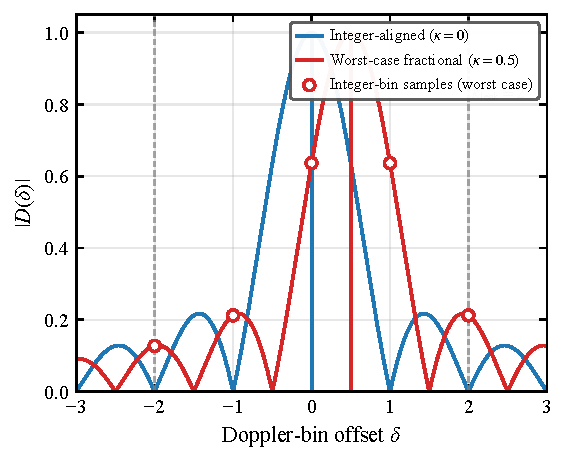
\includegraphics[width=0.55\linewidth]{system_block/fig_dirichlet_kernel.pdf}
\caption{Dirichlet-kernel magnitude $|D(\delta)| = |\sin(\pi\delta) / (\Nsub \sin(\pi\delta / \Nsub))|$ from \eqref{eq:dirichlet} at $\Nsub = 1024$, plotted against the integer-Doppler offset $\delta$. Two cases are overlaid: the integer-aligned residual ($\kappa = k_p^{\text{real}} - k_p = 0$, blue), where the kernel collapses to a sampling indicator and an integer-Doppler dictionary loses no per-path energy; and the worst-case fractional residual ($|\kappa| = 0.5$, red), where the integer-bin samples (red circles) at $\delta \in \{0, +1\}$ each carry $\approx 41\%$ of per-path energy and the samples at $\delta \in \{-1, +2\}$ each carry $\approx 4.4\%$. The dashed vertical lines mark the $\kleak = 2$ truncation boundary used by the simulator; the two-sided sum of squared truncated coefficients beyond $|\delta| > \kleak$ amounts to $\approx 8.3\%$ of per-path energy at $|\kappa| = 0.5$, the figure quoted in the paragraph above. The non-zero side-lobes flanking the kernel peak are the structurally predictable energy that the post-OMP virtual-tap expansion (\S\ref{ssec:joint}) and the learned support-refinement ranker (\S\ref{ssec:c2rel}) are designed to recover.}
\label{fig:dirichlet}
\end{figure}

The geometry summarised in Fig.~\ref{fig:dirichlet} is the physical reason why a single OMP pass on the integer-Doppler dictionary cannot fully resolve the effective channel under fractional Doppler: at the worst-case residual the side-lobe samples adjacent to a main-lobe atom each carry energy comparable to a separate weak path, yet sit at deterministic integer offsets from that already-active atom. This structural predictability motivates the support-refinement head of \S\ref{ssec:c2rel} and is the geometric anchor used by the mechanism discussion in \S\ref{ssec:disc_head}.

\subsection{Superimposed pilot signal model}
\label{ssec:sp}

To preserve spectral efficiency, every chirp-domain sub-carrier simultaneously carries data and pilot energy under a fixed superimposed-pilot (SP) frame
\begin{equation}
\mbx \;=\; \sqrt{\rhop}\; \xp \;+\; \sqrt{1 - \rhop}\; \xd, \qquad \rhop \in (0, 1), \label{eq:sp_frame}
\end{equation}
where $\xp$ is a deterministic Zadoff--Chu sequence of root $r = 7$ and length $\Nsub$ normalised to unit energy~\cite{kaleh2005zadoffchu}, and $\xd$ is a QPSK data vector. The canonical pilot power fraction is $\rhop = 0.5$; higher $\rhop$ strengthens the pilot observation at the cost of data energy, and lower $\rhop$ does the converse~\cite{orozco2011superimposed,tugnait2006superimposed}. Under the model~\eqref{eq:afdm_model}, the pilot projection performed at the receiver yields
\begin{equation}
\xp^H \mby \;=\; \sqrt{\rhop}\; \xp^H \Heff \xp \;+\; \sqrt{1 - \rhop}\; \xp^H \Heff \xd \;+\; \xp^H \mbn, \label{eq:pilot_projection}
\end{equation}
so that the data term $\sqrt{1 - \rhop}\, \xp^H \Heff \xd$ enters as structured interference to the OMP dictionary correlator. Treating $\xd$ as a QPSK data vector independent of $\xp$ with covariance $\E[\xd \xd^H] = (1/\Nsub) \mathbf{I}_{\Nsub}$, the conditional second moment of the interference term given the channel is
\begin{equation}
\E\bigl[\,|\sqrt{1-\rhop}\, \xp^H \Heff \xd|^2\,\big|\,\Heff\bigr] \;=\; (1-\rhop) \cdot \|\Heff^H \xp\|^2 / \Nsub, \label{eq:interferencevar}
\end{equation}
which scales with the channel norm $\|\Heff\|$ and the pilot autocorrelation, and does not shrink with increasing $\snr$. At the canonical operating point ($\rhop = 0.5$, $\Ppath = 8$, $\xp$ a unit-norm Zadoff--Chu sequence) the resulting estimation-limited error floor is observed at $\ber \approx 5 \times 10^{-2}$ for a serial OMP+MP receiver from $\snr \geq 15$~dB; this floor is not derived in closed form because $\|\Heff^H \xp\|^2$ depends on the channel realisation and the pilot--channel cross-correlation structure, and is therefore quantified empirically in Chapter~\ref{sec:results}.

\subsection{Sparse-baseline OMP dictionary}
\label{ssec:dictionary}

The OMP dictionary $\mbPhi \in \C^{\Nsub \times Q}$ is constructed column-wise by evaluating the chirp-domain response of every candidate $(l, k)$-bin in the physical integer search region
\begin{equation}
l \in \{0, 1, \dots, \lmax - 1\}, \qquad k \in \{-\kmax, \dots, \kmax\},
\end{equation}
so that the dictionary size is $Q = (2\kmax + 1) \cdot \lmax$. The dictionary spans physical integer delay--Doppler bins only; the Dirichlet expansion \eqref{eq:dirichlet} is applied post-OMP to each selected atom, so the fractional-Doppler half-width $\kleak$ does not enlarge the dictionary and enters only through the $(2\kleak{+}1)$-fold virtual-tap replication used in the DA-LS refit and MP-BP blocks of \S\ref{ssec:joint}. The caps $\lmax$ and $\kmax$ follow directly from the physical channel parameters,
\begin{align}
\lmax &= \lceil \tau_{\text{spread}} \cdot \fs \rceil, \label{eq:lmax} \\
\kmax &= \left\lceil \frac{v_{\max}\, \fc\, \Nsub}{c\, \fs} \right\rceil, \label{eq:kmax}
\end{align}
and have a consequence that is central to the complexity argument in \S\ref{ssec:complexity}. Holding the sampling rate $\fs$ fixed at the $\fs = 4B$ operating point used throughout this report, $\lmax$ is a constant independent of $\Nsub$, while $\kmax \propto \Nsub / \fs$ grows linearly with $\Nsub$. Therefore
\begin{equation}
Q \;=\; (2\kmax + 1) \cdot \lmax \;=\; \mathcal{O}(\Nsub) \cdot \mathcal{O}(1) \;=\; \mathcal{O}(\Nsub). \label{eq:Qlinear}
\end{equation}
Table~\ref{tab:dictsize} reports the resulting $(\lmax, \kmax, Q)$ triples at $\Nsub \in \{512, 1024, 2048\}$ under the canonical $\fs = 4B$ setting.

\begin{table}[t]
\centering
\caption{OMP dictionary size under the canonical AFDM configuration used throughout this report ($\tau_{\text{spread}} = 10$~ms, $v_{\max} = 3$~m/s, $\fc = 12$~kHz, $\fs = 4B = 16$~kHz). Under the fixed-$\fs$ convention, $\lmax = \lceil \tau_{\text{spread}} \fs \rceil = 160$ is independent of $\Nsub$, while $\kmax = \lceil v_{\max}\fc\Nsub/(c\fs)\rceil$ grows linearly with $\Nsub$. The Chapter~\ref{sec:results} operating point ($\Nsub = 1024$) corresponds to the middle row.}
\label{tab:dictsize}
\begin{tabular}{rrrr}
\toprule
$\Nsub$ & $\lmax$ & $\kmax$ & $Q = (2\kmax+1)\lmax$ \\
\midrule
512  & 160 & 1 & 480   \\
1024 & 160 & 2 & 800   \\
2048 & 160 & 4 & 1\,440 \\
\bottomrule
\end{tabular}
\end{table}

The asymptotic claim $Q = \mathcal{O}(\Nsub)$ is invariant across the two natural UWA conventions: under fixed-$\fs$ as above, and under fixed sub-carrier spacing $\Delta f$ (so that $\fs = \Nsub \Delta f$), in which case $\lmax \propto \Nsub$ and $\kmax = \mathcal{O}(1)$ and the product $Q = (2\kmax{+}1)\lmax = \mathcal{O}(\Nsub)$ still holds. The hidden leading constants differ between the two conventions and are not interchangeable when quoting per-frame multiply-accumulate (MAC) counts.

Each OMP iteration evaluates $\mbPhi^H \mathbf{r}$ at a cost of $\mathcal{O}(\Nsub Q)$ complex multiplications and solves an $s\times s$ least-squares system at $\mathcal{O}(\Nsub s + s^3)$ for the standard direct factorisation, where $s \leq \Ppath$ is the current support size. Running OMP to a target sparsity of $\Ppath = 8$ therefore costs
\begin{equation}
C_{\text{OMP}} \;=\; \mathcal{O}(\Ppath \Nsub Q + \Ppath^4) \;=\; \mathcal{O}(\Ppath \Nsub^2) \label{eq:omp_cost}
\end{equation}
per frame under \eqref{eq:Qlinear}, where the $\Ppath^4$ term is absorbed because $\Ppath \ll \Nsub$ at every operating point used in this report.

\subsection{Joint OMP-once + iterative LS/MP-BP receiver}
\label{ssec:joint}

The receiver performs one OMP support-recovery pass and then iterates only over the data-aided path-gain least-squares (DA-LS) refit and the sparse MP-BP detection block. Algorithm~\ref{alg:joint} summarises the recipe.

\begin{algorithm}[t]
\caption{Classical joint OMP-once + iterative LS/MP-BP receiver.}
\label{alg:joint}
\begin{small}
\textbf{Input}: $\mby$ (chirp-domain received frame), $\mbPhi$ (OMP dictionary), known $\xp$, pilot power $\rhop$. \\
\textbf{Output}: hard-decision data bits $\hat{\xd}$. \\
\textbf{Hyperparameters}: outer iterations $T_\text{out} = 5$, MP inner iterations $T_\text{mp} = 20$, damping $\gamma_h = 0.7$, prune threshold $\tau_h = 10^{-2}\cdot \max |\hat{h}|$.
\begin{enumerate}[leftmargin=*,itemsep=1pt,topsep=2pt]
  \item \textbf{OMP-once}: run orthogonal matching pursuit on $\mbPhi$ with target sparsity $\Ppath$; obtain support $\hat{S}^{(0)}$ and path gains $\hat{\mbh}^{(0)}$. Initialise $\hat{\xd}^{(0)}$ with an LMMSE solution on $\hat{S}^{(0)}$.
  \item \textbf{For} $t = 1, \dots, T_\text{out}$:
  \begin{enumerate}[leftmargin=*,itemsep=1pt,topsep=2pt]
    \item Form the data-cancellation residual
    \begin{equation}
    \mathbf{r}^{(t)} \;=\; \mby \;-\; \sqrt{1-\rhop}\, \Heff(\hat{\mbh}^{(t-1)})\, \hat{\xd}^{(t-1)},
    \label{eq:dals_resid}
    \end{equation}
    where $\hat{\xd}^{(0)}$ is the LMMSE initialisation from step~1; the $\sqrt{\rhop}\,\xp$ pilot contribution is retained in $\mathbf{r}^{(t)}$ because $\xp$ is absorbed into the OMP dictionary $\mbPhi$ (each column carries its pilot-aware atom vector), so the data-interference term is the only component that must be cancelled explicitly.
    \item Damped DA-LS refit on the current support $\hat{S}^{(t-1)}$:
    \begin{equation}
    \hat{\mbh}^{(t)} \;=\; (1-\gamma_h)\,\hat{\mbh}^{(t-1)} \;+\; \gamma_h \cdot \mbPhi_{\hat{S}^{(t-1)}}^{\dagger}\, \mathbf{r}^{(t)}.
    \label{eq:dals}
    \end{equation}
    \item MP-BP on the sparse factor graph $(\Heff(\hat{\mbh}^{(t)}), \mby)$ for $T_\text{mp}$ iterations with damping $0.5$; update posterior means $\hat{\xd}^{(t)}$ and per-symbol variances $\sigma_{d,i}^2$.
    \item Adaptive $\sigma^2$ update; prune atoms with $|\hat{h}_s^{(t)}| < \tau_h$ (always retain the top-$\Ppath$).
  \end{enumerate}
  \item Hard-decide $\hat{\xd} = \mathrm{QPSK\text{-}demap}(\hat{\xd}^{(T_\text{out})})$.
\end{enumerate}
\end{small}
\end{algorithm}

\begin{figure}[t]
\centering
\includegraphics[width=\linewidth]{system_block/figure_a_new.png}
\caption{Classical OMP-once + iterative LS/MP-BP joint receiver (Algorithm~\ref{alg:joint} in block-diagram form). The outer loop (dashed rectangle) runs for $T_\text{out} = 5$ iterations; each iteration forms a data-cancellation residual, refits the path gains on a locked support via damped DA-LS, runs sparse MP-BP detection on the Dirichlet-expanded virtual-tap factor graph, updates the adaptive noise-variance estimate, and prunes the support.}
\label{fig:classical_joint_arch}
\end{figure}

\paragraph{MP-BP messages on the sparse chirp-domain factor graph.}
The data-detection block of Algorithm~\ref{alg:joint} follows the iterative-receiver framework of Wymeersch~\cite{wymeersch2007iterativereceiver} and the factor-graph paradigm surveyed by Kschischang~\emph{et~al.}~\cite{kschischang2001factorgraph}, and is implemented as Gaussian message passing on a bipartite factor graph derived from the pilot-subtracted observation. Subtracting the estimated pilot contribution from~\eqref{eq:afdm_model} yields, for every $j \in \{0, \dots, \Nsub - 1\}$,
\begin{equation}
\tilde{y}_j \;:=\; y_j - \sqrt{\rhop}\, [\Heff(\hat{\mbh}^{(t)})\, \xp]_j \;=\; \sum_{i \in \mathcal{N}(j)} \tilde{H}_{j,i}\, x_{d,i} \;+\; n_j, \label{eq:mpbp_input}
\end{equation}
where $\tilde{H}_{j,i} := \sqrt{1-\rhop}\, [\Heff(\hat{\mbh}^{(t)})]_{j,i}$ absorbs the data-power normalisation and $\mathcal{N}(j) := \{i : \tilde{H}_{j,i} \neq 0\}$ is the index set of variables coupled to factor $j$. The factor graph carries $\Nsub$ variable nodes (one per data symbol $x_{d,i}$) and $\Nsub$ factor nodes (one per row of~\eqref{eq:mpbp_input}). The neighbourhood degree is bounded by $|\mathcal{N}(j)| \leq \Ppath \cdot (2\kleak + 1) = 40$ in the nominal Dirichlet expansion and averages $\preal \approx 28$ per frame after pruning of negligible Dirichlet-weighted entries (App.~\ref{app:recall}); both bounds are constants in $\Nsub$, which is the property that enables $\mathcal{O}(\Nsub)$ per-iteration message passing.

At inner iteration $\ell$, the variable-to-factor message from $x_{d,i}$ to factor $j$ is parameterised as a Gaussian with mean $\mu_{i \to j}^{(\ell)}$ and variance $v_{i \to j}^{(\ell)}$, obtained by aggregating all incoming factor-to-variable messages with the one returning from $j$ excluded:
\begin{equation}
\frac{1}{v_{i \to j}^{(\ell)}} \;=\; \!\sum_{j' \in \mathcal{M}(i) \setminus \{j\}}\! \frac{1}{v_{j' \to i}^{(\ell-1)}}, \qquad \frac{\mu_{i \to j}^{(\ell)}}{v_{i \to j}^{(\ell)}} \;=\; \!\sum_{j' \in \mathcal{M}(i) \setminus \{j\}}\! \frac{\mu_{j' \to i}^{(\ell-1)}}{v_{j' \to i}^{(\ell-1)}}, \label{eq:mpbp_var}
\end{equation}
where $\mathcal{M}(i) := \{j : i \in \mathcal{N}(j)\}$ shares the same constant degree bound. The factor-to-variable message marginalises the row-$j$ Gaussian likelihood over all variables in $\mathcal{N}(j) \setminus \{i\}$,
\begin{align}
\mu_{j \to i}^{(\ell)} &\;=\; \frac{1}{\tilde{H}_{j,i}} \left( \tilde{y}_j - \!\!\sum_{i' \in \mathcal{N}(j) \setminus \{i\}}\!\! \tilde{H}_{j, i'}\, \mu_{i' \to j}^{(\ell)} \right),
\label{eq:mpbp_fact_mean} \\
v_{j \to i}^{(\ell)} &\;=\; \frac{1}{|\tilde{H}_{j,i}|^2} \left( \hat{\sigma}_n^2 + \!\!\sum_{i' \in \mathcal{N}(j) \setminus \{i\}}\!\! |\tilde{H}_{j, i'}|^2\, v_{i' \to j}^{(\ell)} \right), \label{eq:mpbp_fact_var}
\end{align}
where $\hat{\sigma}_n^2$ is the adaptive noise-variance estimate updated at the end of each outer iteration. Both message updates are damped with $\eta = 0.5$ to suppress oscillations on the short cycles characteristic of the Dirichlet-expanded factor graph, $\mu_{i \to j}^{(\ell)} \leftarrow \eta\, \tilde{\mu}_{i \to j}^{(\ell)} + (1-\eta)\, \mu_{i \to j}^{(\ell-1)}$ and analogously for the variances, where $\tilde{\mu}_{i \to j}^{(\ell)}$ denotes the undamped update of~\eqref{eq:mpbp_var}. After $T_\text{mp} = 20$ inner iterations, the posterior on each data symbol is read off by aggregating all incoming factor messages,
\begin{equation}
\frac{1}{\sigma_{d,i}^2} \;=\; \!\sum_{j \in \mathcal{M}(i)}\! \frac{1}{v_{j \to i}^{(T_\text{mp})}}, \qquad \frac{\hat{x}_{d,i}}{\sigma_{d,i}^2} \;=\; \!\sum_{j \in \mathcal{M}(i)}\! \frac{\mu_{j \to i}^{(T_\text{mp})}}{v_{j \to i}^{(T_\text{mp})}}, \label{eq:mpbp_post}
\end{equation}
followed by a Gray-coded QPSK projection $\hat{x}_{d,i} \mapsto \mathrm{QPSK\text{-}demap}(\hat{x}_{d,i})$ that returns the hard-decision data symbol. The Gaussian approximation maintained throughout the inner loop is the standard soft-Gaussian belief-propagation form for finite-alphabet symbols~\cite{wymeersch2007iterativereceiver}, with the QPSK constraint enforced only at the final projection. Because $|\mathcal{N}(j)|$ and $|\mathcal{M}(i)|$ are bounded by constants independent of $\Nsub$, each inner iteration evaluates $\mathcal{O}(\preal \cdot \Nsub)$ scalar updates across all factor and variable nodes, so the data-detection block costs $\mathcal{O}(T_\text{mp} \Nsub)$ per outer iteration. This is the source of the $\mathcal{O}(T_\text{mp} \Nsub)$ term in the per-frame budget of~\eqref{eq:classcomplex}, and it is two orders of magnitude cheaper than a chirp-domain dense MMSE equaliser's $\mathcal{O}(\Nsub^3)$ at $\Nsub = 1024$.

Four design choices in Algorithm~\ref{alg:joint} are central to the receiver's behaviour, and each rejects a simpler or more expensive alternative on empirical or analytical grounds. The OMP-once choice rests on a stability observation: the empirical support Jaccard between successive OMP passes in a hypothetical full re-OMP schedule exceeds $0.94$ from iteration~2 onwards (Fig.~\ref{fig:iterconv}), so the atoms within the support are already stable after a single pass and the only quantity that continues to evolve is the per-path gain amplitude. Chapter~\ref{sec:results}~(\S\ref{ssec:probes}) confirms this independently: OMP-once recovers a mean $\approx 95\%$ recall against the effective Dirichlet-expanded virtual-tap oracle support across all training SNRs (Table~\ref{tab:supportrecall}), so a second OMP pass has nothing new to find. Re-running OMP across outer iterations therefore re-solves a near-identical atom-selection problem $T_\text{out} = 5$ times per frame at a constant-factor overhead of $\sim 5\times$~\eqref{eq:omp_cost} without any change in asymptotic class. Once the support is locked, the path gains are refined by a damped DA-LS update rather than a full LS solve: a full LS over the unrestricted dictionary would amplify noise from unexplored columns, whereas the DA-LS refit \eqref{eq:dals} on the locked support uses exactly the $\Ppath \approx 8$ physical (or $\approx 28$ virtual) taps from step~1 and keeps the gain-update cost at $\mathcal{O}(\Ppath^2 \Nsub)$.

The detection block is sparse MP-BP rather than a dense chirp-domain equaliser. The factor graph induced by $\Heff(\hat{\mbh}^{(t)})$ carries at most $\Ppath \cdot (2\kleak+1) = 40$ non-trivial symbol-to-symbol edges per row in the nominal Dirichlet expansion, with the empirical effective edge count after pruning of negligible Dirichlet weights averaging $\approx 28$ per frame (App.~\ref{app:recall}, $p_{\text{real}}$); the count is constant in $\Nsub$, so each MP-BP iteration costs $\mathcal{O}(\Nsub)$, against the $\mathcal{O}(\Nsub^3)$ per frame of a dense MMSE equaliser --- two full orders of magnitude more expensive at $\Nsub = 1024$. The choice of SP over an embedded-pilot frame is, finally, the source of the data-interference term that motivates iteration in the first place: under EP the OMP step is clean but the spectral efficiency drops by a factor proportional to the pilot fraction, and in a UWA context guard regions also produce artefacts on Dirichlet-expanded virtual taps; SP preserves full data capacity at the cost of the structured interference term \eqref{eq:pilot_projection}, which the iterative recipe is specifically designed to attenuate via successive hard-decision feedback.

\subsection{Learned support-refinement head}
\label{ssec:c2rel}

Even with iteration, the classical joint receiver retains a residual support-selection gap at high SNR, where OMP occasionally misses weak but non-negligible Dirichlet-leakage atoms (typically at $\pm 1$-bin Doppler offsets around the integer-$\kmax$ index) whose estimated gains fall just below $\tau_h$ and are pruned by the gain-magnitude rule. This gap is closed by the \LearnedHead{}: a 1\,041-parameter deep-unfolding module that scores off-support candidates against the currently active support and appends the highest-ranked $\Kadd$ atoms at the initialisation step ($t = 0$), immediately after OMP-once and before the iterative LS/MP-BP loop begins (Fig.~\ref{fig:pipeline_integration}).

\begin{figure}[t]
\centering
\includegraphics[width=\linewidth]{system_block/figure_b_new.png}
\caption{Integration of the learned support-refinement head into the classical OMP-once + iterative LS/MP-BP receiver. The learned block (dark blue) is invoked twice at the initialisation step ($t = 0$), immediately after OMP-once and before the iterative LS/MP-BP loop begins; it ranks the top-$M = 96$ off-support candidates and appends the top-$\Kadd$ atoms to the support. All other blocks are identical to Fig.~\ref{fig:classical_joint_arch}: the head replaces neither OMP-once nor the iterative LS/MP-BP block. The detailed head architecture is given in Fig.~\ref{fig:head_arch}.}
\label{fig:pipeline_integration}
\end{figure}

\begin{figure}[t]
\centering
\includegraphics[width=\linewidth]{system_block/figure_c_new.png}
\caption{Learned support-refinement head (architecture). Two parallel inputs per candidate $i$: a 7-D self-feature $\mathbf{u}_i$ and a set of 6-D pair features $\{\mathbf{v}_{i,s}\}_{s \in \hat{S}}$ indexed over the current active support $\hat{S}$. The shared pair-encoder ($\mathbb{R}^6 \!\to\! \mathbb{R}^{16} \!\to\! \mathbb{R}^{16}$, 384 parameters) is applied element-wise over $(i, s)$ pairs; order-invariant pooling (concat of channel-wise max and mean over $s \in \hat{S}$) produces a 32-D pair descriptor per candidate, which is concatenated with $\mathbf{u}_i$ to form $\boldsymbol{\phi}_i \in \mathbb{R}^{39}$. The shared scorer ($\mathbb{R}^{39} \!\to\! \mathbb{R}^{16} \!\to\! \mathbb{R}^1$, 657 parameters) emits a scalar logit $s_i$; the deterministic top-$\Kadd$ ranker selects the atoms to append. Total trainable parameters: $384 + 657 = 1\,041$. The logits are used only for ranking.}
\label{fig:head_arch}
\end{figure}

\paragraph{Features.}
Let $M$ denote the number of off-support candidate atoms at iteration~$t$; the deployed receiver fixes $M = 96$ by retaining the top-$96$ residual-correlation candidates. For each candidate $i \in \{1, \dots, M\}$ a 7-dimensional self-feature $\mathbf{u}_i \in \R^{7}$ is constructed from
\begin{enumerate}[leftmargin=*,itemsep=0pt,topsep=1pt]
  \item the log matched-filter magnitude $\log |\mbPhi_i^H \mathbf{r}^{(t)}|$;
  \item the margin to the weakest active atom, $\log |\mbPhi_i^H \mathbf{r}^{(t)}| - \min_{s \in \hat{S}} \log |\hat{h}_s|$;
  \item the normalised delay bin index $l_i / \lmax$;
  \item the normalised Doppler bin index $(k_i + \kmax) / (2\kmax)$;
  \item the residual projection norm $\|\mbPhi_i^H \mathbf{r}^{(t)}\| / \|\mathbf{r}^{(t)}\|$;
  \item the candidate rank among the $M$ atoms, normalised to $[0, 1]$;
  \item a binary flag indicating whether $(l_i, k_i)$ lies within $\kleak$ Doppler bins of some active atom (Dirichlet-leakage neighbour).
\end{enumerate}
For each (candidate, active atom) pair $(i, s)$ a 6-dimensional pair feature $\mathbf{v}_{i,s} \in \R^{6}$ is computed:
\begin{equation}
\mathbf{v}_{i,s} =
\bigl[
l_i-l_s,\;
k_i-k_s,\;
\log |\hat{h}_s|,\;
|\mbPhi_i^H \mbPhi_s|,\;
\frac{\|(l_i-l_s,\; k_i-k_s)\|_2}{\lmax + 2\kmax},\;
\frac{|\hat{h}_s|}{\max_{s'} |\hat{h}_{s'}|}
\bigr].
\label{eq:pairfeature}
\end{equation}

\paragraph{Feature design rationale.}
The 7-dimensional self-feature and 6-dimensional pair feature are organised as three complementary information channels that the scorer needs in order to discriminate Dirichlet side-lobe atoms from noise-driven candidates. Self-features 1, 2, and 5 expose the candidate's data-driven correlation strength against three different normalisations: the absolute matched-filter magnitude $\log|\mbPhi_i^H \mathbf{r}^{(t)}|$, the margin against the weakest active atom $\log|\mbPhi_i^H \mathbf{r}^{(t)}| - \min_{s \in \hat{S}} \log|\hat{h}_s|$ that places the candidate on the same logarithmic axis as the active support's tail, and the residual-normalised projection $\|\mbPhi_i^H \mathbf{r}^{(t)}\|/\|\mathbf{r}^{(t)}\|$ that controls for the overall residual energy at iteration $t$. Self-features 3 and 4, the normalised delay and Doppler indices $l_i / \lmax$ and $(k_i + \kmax)/(2\kmax)$, locate the candidate on the physical lattice and let the scorer learn position-dependent priors --- for instance, that bins near $\pm \kmax$ are more likely to host fractional-leakage residuals than bins near zero. Self-feature 6, the candidate's rank among the $M = 96$ retained atoms, provides a tie-breaker that lets the scorer condition on whether a candidate sits near the top of the matched-filter shortlist or at its tail. Self-feature 7, the binary indicator that $(l_i, k_i)$ lies within $\kleak$ Doppler bins of an active atom, is the most directly mechanism-coupled feature: it flags the geometric signature of a Dirichlet side-lobe neighbour and is the feature that most cleanly distinguishes the high-SNR exploitable regime from the low-SNR noise-dominated regime developed in \S\ref{ssec:disc_head}.

The 6-dimensional pair feature $\mathbf{v}_{i,s}$ extends the same reasoning to the relational structure between candidate $i$ and each active atom $s$. The integer offsets $(l_i - l_s, k_i - k_s)$ are the direct encoding of the $(\Delta l, \Delta k) = (0, \pm 1)$ Dirichlet side-lobe signature; combined with the active atom's log-gain $\log|\hat{h}_s|$ and its gain prominence $|\hat{h}_s| / \max_{s'}|\hat{h}_{s'}|$, they let the scorer learn that a candidate at $(0, \pm 1)$ offset from a high-gain active atom is far more likely to be a side-lobe than the same candidate at the same offset from a weak active atom. The pair correlation $|\mbPhi_i^H \mbPhi_s|$ measures dictionary-column similarity directly and supplements the integer-offset signal with a continuous coherence measure, so that pairs of atoms whose chirp-domain responses overlap geometrically can be flagged even when the integer-offset pattern is ambiguous. The normalised Euclidean distance $\|(l_i - l_s,\, k_i - k_s)\|_2 / (\lmax + 2\kmax)$ provides a single scalar that the order-invariant pooling of the architecture (described next) can aggregate across all $|\hat{S}|$ active atoms without losing the geometric information. Taken together, the feature design encodes the rule that a candidate should be promoted when it is a low-Hamming-distance Doppler neighbour of an active atom of non-trivial gain and when its matched-filter response sits above the active-set tail; this is the rule that the oracle-headroom analysis of \S\ref{ssec:probes} validates as covering the bulk of the achievable support-refinement gap, and it is the rule that the scorer is trained to recover.

\paragraph{Architecture.}
The head consists of a shared pair encoder followed by a per-candidate scorer. The pair encoder, denoted $f_{\text{pair}}: \R^{6} \to \R^{16} \to \R^{16}$ with SiLU activation~\cite{elfwing2018silu} after each linear layer, is applied element-wise to every pair feature $\mathbf{v}_{i,s}$, contributing $(6 \cdot 16 + 16) + (16 \cdot 16 + 16) = 384$ parameters. For each candidate $i$, the resulting set of $|\hat{S}|$ per-pair 16-vectors is aggregated into a 32-dimensional pair descriptor by concatenating the element-wise maximum and the element-wise mean across $s$, with no additional trainable parameters. The pooled descriptor is concatenated with the 7-dimensional self-feature $\mathbf{u}_i$ to form a 39-dimensional vector and passed through the scorer $f_{\text{score}}: \R^{39} \to \R^{16} \to \R^{1}$ (SiLU after the first linear; zero-initialised output weights; output bias initialised at $-8$), contributing $(39 \cdot 16 + 16) + (16 \cdot 1 + 1) = 657$ parameters. The total trainable parameter count is $384 + 657 = 1\,041$, of which $\approx 37\%$ sit in the pair encoder and $\approx 63\%$ in the scorer.

\paragraph{Inference.}
The head is deployed as a deterministic fixed-budget top-$\Kadd$ ranker with $\Kadd = 4$: the scorer logits rank the $M = 96$ off-support candidates on every frame, and the top $\Kadd = 4$ logits are appended to the active support without any per-candidate probability thresholding. At outer iteration $t = 0$ the head is invoked twice (i.e.\ two refinement rounds), with support-pruning deferred until the final outer iteration and the two most recently appended atoms protected from gain-prune; hard-decision symbol feedback is used throughout. The learned final-scorer bias ($\approx -8$) is replaced by $+10$ at inference time so that the top-$\Kadd$ selection always fires, which is mathematically a ranking-preserving threshold shift; the deployment is therefore described as ranking-only rather than as a probability-calibrated detector. The training-objective and inference-objective alignment that this introduces is discussed in \S\ref{ssec:training} and Chapter~\ref{sec:discussion}.

\subsection{Training}
\label{ssec:training}

Per-frame feature caches are harvested by running the classical joint receiver to completion on $(\mathrm{channel}, \mathrm{data}, \mathrm{noise})$ realisations drawn from a dedicated training seed block. Each cached frame carries, per candidate, a binary supervision label $y_i \in \{0, 1\}$ that equals $1$ iff the candidate $(l_i, k_i)$ coincides with an active Dirichlet-weighted ground-truth virtual tap of the true channel. The positive-class rate over the $M = 96$ candidates is $\approx 3\%$, which skews the binary cross-entropy (BCE) objective toward the negative class and accounts for the learned final-scorer bias drifting toward $-8$.

The loss is a weighted sum of per-candidate BCE and a pairwise ranking hinge,
\begin{equation}
\mathcal{L}(\theta) \;=\; \mathcal{L}_{\text{BCE}}(\theta) \;+\; \lambda_{\text{rank}} \cdot \max\bigl(0,\; 1 - \min_{y_i=1} s_i(\theta) + \max_{y_j=0} s_j(\theta)\bigr), \qquad \lambda_{\text{rank}} = 0.5, \label{eq:loss}
\end{equation}
where $s_i(\theta)$ is the scorer logit for candidate $i$ and $\theta$ are the head parameters. Training uses AdamW~\cite{loshchilov2019adamw} with learning rate $10^{-3}$, weight decay $10^{-4}$, batch size $512$ cached frames, for 8 epochs with early stopping on the validation BCE (patience = 2). The cache is split 90/10 frame-level into train/val at fixed seed $13\,579$.

The training cache used for the deployed checkpoint is a 27\,k-frame 4-SNR cache at $\snr \in \{10, 15, 20, 25\}$~dB with per-SNR frame weights $\{0.2, 0.3, 0.3, 0.2\}$, harvested at the $\fs = 4B$ operating point. Covering $\snr = 25$~dB explicitly in the cache is necessary to avoid a slight regression in the head's high-SNR behaviour at the same operating point.

\paragraph{Ranking-only deployment.}
Although the BCE term in \eqref{eq:loss} would in principle support a probability-calibrated interpretation of the scorer output, the deployed head is used purely as a top-$\Kadd$ ranker. The bias-replacement scheme at inference is rank-preserving: writing the final logit as $s_i = z_i + b$, replacing $b_{\text{learned}} \approx -8$ by $b_{\text{patch}} = +10$ is a uniform translation of every candidate's logit, which leaves the top-$\Kadd$ ordering invariant. The patch's only operational effect is to shift the gate threshold from $z_i > 8$ (rarely satisfied under $b_{\text{learned}}$) to $z_i > -10$ (almost always satisfied), so every frame proceeds to a forced top-$\Kadd$ selection rather than to a no-op gate output. Probability calibration of the scores is out of scope. A principled alternative that aligns training and inference --- a differentiable top-$\Kadd$ loss or a listwise ranking loss --- is identified as future work in Chapter~\ref{sec:conclusion}. The full analytical decomposition of the bias patch into its rank-preservation and gate-toggling components is deferred to App.~\ref{app:topk_patch}.

\subsection{Complexity analysis}
\label{ssec:complexity}

The arithmetic cost of the proposed receiver is the sum of the classical joint cost and the learned-head overhead. From \S\ref{ssec:joint}, the classical joint costs
\begin{equation}
C_{\text{classical}} \;=\; \underbrace{\mathcal{O}(\Ppath \Nsub Q)}_{\text{OMP-once}} \;+\; T_\text{out} \cdot \bigl[\,\mathcal{O}(\Ppath^2 \Nsub)\ \text{DA-LS}\,+\,\mathcal{O}(T_\text{mp} \Nsub)\ \text{MP-BP}\,\bigr] \;=\; \mathcal{O}(\Ppath \Nsub^2) \label{eq:classcomplex}
\end{equation}
per frame, using $Q = \mathcal{O}(\Nsub)$ from \eqref{eq:Qlinear}. The learned head, per refinement round, performs four operations of order $\Nsub$:
(i) candidate-pool selection by computing the residual--dictionary correlation $\mbPhi^H \mathbf{r}$ over the full $Q$-column dictionary at $\mathcal{O}(\Nsub Q)$ and retrieving the top-$M$ off-support candidates by argpartition at $\mathcal{O}(Q)$ (this step is reused if the OMP-once correlation vector is cached across head invocations, otherwise paid once per round);
(ii) $M$ residual projections $\mbPhi_i^H \mathbf{r}$ at $\mathcal{O}(\Nsub)$ each;
(iii) $M \cdot \Ppath$ pair inner products $\mbPhi_i^H \mbPhi_s$ at $\mathcal{O}(\Nsub)$ each, used in the pair feature \eqref{eq:pairfeature};
(iv) $\mathcal{O}(M \Ppath)$ pair-encoder evaluations and $\mathcal{O}(M)$ scorer evaluations of constant per-pair cost.
Summed over the two refinement rounds,
\begin{equation}
C_{\text{head}} \;=\; \mathcal{O}\bigl(\Nsub Q + M \Ppath \Nsub\bigr) \;=\; \mathcal{O}(\Nsub^2) \label{eq:headcomplex}
\end{equation}
under fixed $(M, \Kadd, \Ppath)$ and $\eqref{eq:Qlinear}$, the same asymptotic class as a single OMP-once matched-filter sweep.

The proposed receiver therefore lies in the same $\mathcal{O}(\Ppath \Nsub^2)$ arithmetic class as the sparse classical baseline, and is two orders of magnitude cheaper than a dense LMMSE channel estimator ($\mathcal{O}(\Nsub^3)$) and a $5\times$ constant factor cheaper than a re-OMP-per-iteration schedule. Table~\ref{tab:complexity} in Chapter~\ref{sec:results} tabulates per-frame MAC counts at $\Nsub = 1024$ for these recipes; the proposed learned receiver adds $\approx 1.5$~M MAC on top of the $18.6$~M-MAC classical core, for a relative overhead of $\approx 8\%$. The MAC count is a first-order arithmetic measure; runtime, memory-hierarchy, and energy effects on a realistic embedded target are out of scope here and are discussed in \S\ref{ssec:weaknesses}.

\subsection{Evaluation protocol}
\label{ssec:eval}

All receivers are evaluated under a strict paired-frame protocol. For every $\snr$ point, each of the four receivers (\Serial{}, \ClassicalJoint{}, \LearnedHead{}, \Oracle{}) consumes the same $(\mathrm{channel}, \mathrm{data}, \mathrm{noise})$ realisation drawn from an RNG chained off a master seed (default $20\,260\,425$), so that BER differences across receivers are interpretable frame-by-frame and invariant to channel-draw variance. The default bit budget is $400$~frames~$\times\,2 \cdot 1024 = 8.19 \times 10^{5}$~bits per $\snr$ point.

Reported BERs are observed frequencies $\hat{p} = \text{bit errors}/\text{bits}$. For the headline numbers at $\fs = 4B$, two-sided Clopper--Pearson 95\% confidence intervals are quoted from the exact binomial distribution. Significance between the classical joint and the learned receiver is tested with the continuity-corrected paired McNemar $\chi^2$ on bit-level discordant counts $(n_{10}, n_{01})$; the reported $p$-values are the two-sided asymptotic values, with the within-frame independence assumption, the one-sided exact-binomial complement, and the degenerate-discordants edge case discussed in Appendix~\ref{app:mcnemar}. Where the Monte-Carlo sampling uses an adaptive early-stop rule, the sampler terminates an $\snr$ point only after the classical arm has accumulated a target bit-error budget and a minimum frame count, so the recorded bit budget per point is never smaller than the budget required to make the paired test well-defined.

Train, validation, and test separation is enforced at the seed level. The $\fs = 4B$ feature cache is produced from training seed blocks $20\,260\,420$ and $20\,260\,421$, while all evaluation frames are drawn from a pairwise disjoint set of evaluation seeds: the 3-seed pooled headline in Table~\ref{tab:ber4b} uses evaluation seed blocks $20\,260\,423$, $20\,260\,424$, $20\,260\,425$, and the single-seed illustrative row uses the isolated master seed $20\,260\,425$. Training and evaluation seed blocks are pairwise disjoint by construction; no evaluated $(\mathrm{channel}, \mathrm{data}, \mathrm{noise})$ triple coincides with any training cache frame.

\subsection{Baseline selection and fairness}
\label{ssec:fairness}

Four receivers are compared head-to-head in Chapter~\ref{sec:results}. The \Serial{} arm is the closest single-pass realisation of the classical sparse-recovery literature~\cite{tropp2007signal,berger2010uwasparse} and makes the SP estimation-limited floor explicit. The \ClassicalJoint{} arm is the strongest classical baseline for AFDM-SP that this report constructs; it shares every component with \LearnedHead{} except the head itself, which is precisely the asymmetry needed to attribute observed gains to the learned module. The \Oracle{} arm uses the true $\Heff$ with pilot cancellation and a dense MMSE equaliser as a reference rather than as an information-theoretic lower bound (\S\ref{ssec:weaknesses}).

All four receivers use identical master seeds, identical pilot sequences, identical frame budgets, and identical hyperparameters where applicable: in particular, the classical joint arm is the ablated learned receiver with its head disabled (zero appended atoms and head-logits set to $-\infty$). The only training-time asymmetry is that \LearnedHead{} has seen cached frames at $\snr \in \{10, 15, 20, 25\}$~dB; evaluation points at $\snr \in \{0, 5\}$~dB therefore lie outside the training distribution and are read as out-of-distribution checks rather than in-distribution comparisons. This asymmetry is declared at every table and figure where low-SNR numbers appear.

\section{Results}
\label{sec:results}

This chapter reports four experiments evaluating the proposed receiver. Experiment~1 (\S\ref{ssec:exp1}) measures the BER waterfall and channel-estimation NMSE of all four receivers under the paired-frame protocol of \S\ref{ssec:eval}. Experiment~2 (\S\ref{ssec:iterconv}) studies the convergence of the iterative joint receiver across outer iterations and verifies the choice of $T_\text{out} = 5$ in Algorithm~\ref{alg:joint}. Experiment~3 (\S\ref{ssec:probes}) reports two analyses that ground the learned head's BER contribution in measurable support-selection statistics. Experiment~4 (\S\ref{ssec:complexity_results}) tabulates per-frame multiply-accumulate counts across the receivers and their hypothetical alternatives.

\subsection{Simulation parameters}
\label{ssec:simparams}

Table~\ref{tab:simparams} summarises the physical and algorithmic parameters used for every experiment in this chapter. All BER observations reported below are obtained at the $\fs = 4B$ oversampled rate. Although raising the sampling rate from $2B$ to $4B$ does not shrink the OMP dictionary --- the delay cap $\lmax = \lceil \tau_{\text{spread}} \fs \rceil$ doubles while the Doppler cap $\kmax$ halves, so $Q$ changes from $720$ to $800$ at the canonical parameters --- it produces a finer integer Doppler grid that reduces the typical fractional-Doppler residual per physical path, and improves the matched-filter contrast between true atoms and data-interference atoms; the measured NMSE and BER consequences are visible in Fig.~\ref{fig:ber4b}, and the physical-layer rationale is developed in \S\ref{ssec:disc_oversampling}.

\begin{table}[t]
\centering
\caption{Simulation parameters. One configuration is used for every receiver in every experiment.}
\label{tab:simparams}
\resizebox{\linewidth}{!}{%
\begin{tabular}{ll}
\toprule
\textbf{Parameter} & \textbf{Value} \\
\midrule
Number of sub-carriers $\Nsub$ & 1024 \\
Sub-carrier spacing $\Delta f$ & 15~Hz \\
Carrier frequency $\fc$ & 12~kHz \\
Bandwidth $B$ & 4~kHz \\
Sampling rate $\fs$ & $4B = 16$~kHz \\
Number of physical paths $\Ppath$ & 8 \\
Delay spread $\tau_{\text{spread}}$ & 10~ms (exponential PDP, $\tau_{\text{mean}} = 0.8$~ms) \\
Per-path velocity $v$ & $\mathcal{N}(2, 0.5^2)$~m/s \\
Dirichlet half-width $\kleak$ & 2 ($\Rightarrow$ 5 virtual taps per physical path) \\
Modulation & QPSK, Gray demapping \\
Pilot power fraction $\rhop$ & 0.5 \\
Pilot sequence & Zadoff--Chu with root $r = 7$, length $\Nsub$ \\
Outer iterations $T_\text{out}$ & 5 \\
MP-BP inner iterations $T_\text{mp}$ & 20 \\
OMP dictionary $(\lmax, \kmax, Q)$ & $(160, 2, 800)$ at $\fs = 4B$ \\
\bottomrule
\end{tabular}
}
\end{table}

\subsection{Experiment 1 --- main 4\,B BER waterfall and paired BER reductions}
\label{ssec:exp1}

Fig.~\ref{fig:ber4b} plots the paired-frame BER (left panel) and channel-estimation NMSE (right panel) for the four receivers at $\fs = 4B$. Table~\ref{tab:ber4b} reports the corresponding pooled paired-BER reductions of \LearnedHead{} relative to \ClassicalJoint{} across three independent evaluation-seed blocks, with paired McNemar $p$-values where both arms are above the finite-sample floor and Clopper--Pearson $95\%$ confidence intervals at high SNR. The deployed learned head is the 1\,041-parameter checkpoint trained on the 27\,k-frame 4-SNR cache of \S\ref{ssec:training}.

\begin{figure}[t]
\centering
\includegraphics[width=0.96\linewidth]{loop13/loop13_combined_4B_ber_mse.png}
\caption{Main 4\,B BER waterfall (left) and channel-estimation NMSE (right) at $\fs = 4B$ for the four receivers described in \S\ref{ssec:fairness}. The \LearnedHead{} line is produced by the 27\,k-frame 4-SNR retrained checkpoint. The \Serial{} arm saturates from $\snr \geq 15$~dB; the \ClassicalJoint{} and \LearnedHead{} arms continue to descend, with \LearnedHead{} consistently below \ClassicalJoint{} in the high-SNR region. The \Oracle{} curve is a PCSI+MMSE reference, not an information-theoretic lower bound.}
\label{fig:ber4b}
\end{figure}

\begin{table}[t]
\centering
\caption{4\,B BER waterfall under the paired-frame protocol, pooled across three independent evaluation-seed blocks (seeds $20\,260\,423$/$424$/$425$; adaptive frame counts 600/773/1\,300 at $\snr = 20/25/30$~dB, driven by the error-budget early-stop rule of \S\ref{ssec:eval}). Column $\Delta$ is the relative paired-BER change of \LearnedHead{} against \ClassicalJoint{}, with McNemar $p$-values where both arms are above the finite-sample floor. CP = Clopper--Pearson $95\%$ confidence interval. \emph{Provenance note.} The pooled relative reductions $-37.74/-40.15/-37.59\%$ at $\snr = 20/25/30$~dB (rounded to $-37.7/-40.2/-37.6\%$ in the table for compactness) reproduce exactly from the paired McNemar $n_{10}/n_{01}$ counts of three committed seed-block runs (\texttt{outputs\_loop12\_r3\_official}, \texttt{outputs\_loop12\_seed2\_s20\_s25\_s30}, \texttt{outputs\_loop12\_matched\_f2p\_s20\_30}) via the auditor-friendly committed aggregation script \texttt{afdm\_sp\_joint\_unrolled/scripts/aggregate\_pooled\_pairedeval.py}; canonical output is committed as \texttt{scripts/pooled\_paired\_eval\_4B\_table\_ber4b.md}. The absolute BER columns are derived from the same operating point ($\Nsub = 1024$, $\Ppath = 8$, $\fs = 4B$, ZC pilot $r=7$, $\rhop = 0.5$); a single committed JSON containing the absolute pooled 4B-BERs at all five SNRs is one of the deferred artefacts noted in \S\ref{ssec:weaknesses} (last item).}
\label{tab:ber4b}
\small
\resizebox{\linewidth}{!}{%
\begin{tabular}{rrrrrrll}
\toprule
SNR~(dB) & \Serial{} & \ClassicalJoint{} & \LearnedHead{} & \Oracle{} & $\Delta$ learned vs classical & Raw counts / bits (learned) & CP 95\% CI for \LearnedHead{} \\
\midrule
10  & $7.1 \times 10^{-2}$  & $4.8 \times 10^{-2}$ & $4.5 \times 10^{-2}$ & $2.2 \times 10^{-2}$  & $-2.2\%$ & -- & -- \\
15  & $4.3 \times 10^{-2}$  & $1.9 \times 10^{-2}$ & $1.7 \times 10^{-2}$ & $7.4 \times 10^{-3}$  & $-7.4\%$ ($p < 10^{-6}$) & -- & -- \\
20  & $4.1 \times 10^{-2}$  & $5.0 \times 10^{-4}$ & $\mathbf{3.1 \times 10^{-4}}$ & $1.2 \times 10^{-4}$ & $\mathbf{-37.7\%}$ ($p < 10^{-6}$; 600 paired frames) & $\approx 381 / 1.23 \times 10^{6}$  & $[2.8\times10^{-4}, 3.4\times10^{-4}]$ \\
25  & $4.1 \times 10^{-2}$  & $1.0 \times 10^{-4}$ & $\mathbf{6.0 \times 10^{-5}}$ & $0$ (censored, CP~95\% UB $3.2 \times 10^{-6}$) & $\mathbf{-40.2\%}$ ($p < 10^{-6}$; 773 paired frames) & $\approx 95 / 1.58 \times 10^{6}$  & $[4.8\times10^{-5}, 7.4\times10^{-5}]$ \\
30  & $4.1 \times 10^{-2}$  & $1.8 \times 10^{-5}$ & $\mathbf{1.1 \times 10^{-5}}$ & $0$ (censored, CP~95\% UB $1.4 \times 10^{-6}$) & $\mathbf{-37.6\%}$ ($p < 10^{-6}$; 1\,300 paired frames) & $\approx 29 / 2.66 \times 10^{6}$  & $[7.4\times10^{-6}, 1.6\times10^{-5}]$ \\
\bottomrule
\end{tabular}
}
\end{table}

The \Serial{} arm is estimation-limited from $\snr = 15$~dB onwards on every evaluation seed, with its channel-estimation NMSE frozen at $\approx -11.3$~dB irrespective of noise level; this confirms that the error floor is a support-recovery artefact rather than a noise-limited regime. The \ClassicalJoint{} arm descends monotonically under iteration and, by $\snr = 25$~dB, recovers approximately two to three orders of magnitude of BER relative to \Serial{}, which is the quantitative form of the statement that iteration on a support fixed at the first OMP estimate is sufficient to dismantle the SP interference. Above this baseline the learned head sits strictly below \ClassicalJoint{} at every $\snr$ and opens a consistent visible $\approx 2$~dB paired separation at the three high-SNR points where both arms are above the finite-sample floor: pooled relative BER reductions of $-37.7\%$ at $20$~dB, $-40.2\%$ at $25$~dB, and $-37.6\%$ at $30$~dB, all with continuity-corrected paired McNemar $p$-values well below $10^{-6}$ (Appendix~\ref{app:mcnemar}). At $\snr \leq 10$~dB the pooled gain falls within $3\%$ relative, which is the designed behaviour of a support-refinement module in the noise-limited regime and is examined mechanistically in \S\ref{ssec:disc_head}. At the highest-SNR point of the headline ($\snr = 30$~dB), the pooled observation over $\approx 2.66 \times 10^{6}$ tested bits is $29$ bit errors for the learned head ($1.1 \times 10^{-5}$; CP $95\%$ CI $[7.4 \times 10^{-6},\, 1.6 \times 10^{-5}]$), while the \Oracle{} reference yields $0$ errors in a comparable budget (CP $95\%$ upper bound $1.4 \times 10^{-6}$); the learned arm therefore sits within one order of magnitude of the censoring-bounded reference within this tested bit budget; a tighter ordering would require a $\geq 10\times$ larger bit budget at $\snr = 30$~dB to discriminate the learned arm from the censored-zero oracle.

\subsection{Experiment 2 --- outer-iteration convergence}
\label{ssec:iterconv}

The choice $T_\text{out} = 5$ in Algorithm~\ref{alg:joint} is justified empirically here by tracing the per-iteration BER and verifying that the iterative joint recipe saturates within the chosen iteration budget. Fig.~\ref{fig:iterconv} plots BER against the outer-iteration index $t \in \{1, \dots, 5\}$ at $\snr \in \{15, 20\}$~dB for both the classical joint and learned receivers; the corresponding numerical values are listed in Table~\ref{tab:iterconv}.

\begin{figure}[t]
\centering
\includegraphics[width=0.78\linewidth]{loop13/loop13_iter_convergence_4B.png}
\caption{Outer-iteration convergence at $\snr \in \{15, 20\}$~dB, $\fs = 4B$, with 80 paired frames per $(t, \snr\!=\!15\,\text{dB})$ cell and 300 paired frames per $(t, \snr\!=\!20\,\text{dB})$ cell. Both recipes descend rapidly over $t = 1, \dots, 4$ and saturate by $t = 4$. The classical $t = 4 \!\to\! 5$ move at $\snr = 20$~dB ($8.81 \times 10^{-4} \!\to\! 9.07 \times 10^{-4}$, $+3\%$) sits within $1\sigma$ of a $614{,}400$-bit binomial count; the learned $t = 4 \!\to\! 5$ move ($4.51 \times 10^{-4} \!\to\! 5.42 \times 10^{-4}$, $+20\%$, $\approx 3\sigma$) is consistent with a residual saturation--counting-noise interaction rather than an iteration blow-up. Numerical values in Table~\ref{tab:iterconv}.}
\label{fig:iterconv}
\end{figure}

\begin{table}[t]
\centering
\caption{Per-iteration BER at $\fs = 4B$: 80~frames per $(t, \snr\!=\!15\,\text{dB})$ cell and 300 frames per $(t, \snr\!=\!20\,\text{dB})$ cell. The retrained learned-head checkpoint is deployed at inference under the standard ranking-only configuration of \S\ref{ssec:c2rel}.}
\label{tab:iterconv}
\small
\resizebox{\linewidth}{!}{%
\begin{tabular}{rrrrr}
\toprule
Outer iter $t$ & SNR~=~15~dB \ClassicalJoint{} & SNR~=~15~dB \LearnedHead{} & SNR~=~20~dB \ClassicalJoint{} & SNR~=~20~dB \LearnedHead{} \\
\midrule
1 & $9.11 \times 10^{-2}$ & $8.41 \times 10^{-2}$ & $8.69 \times 10^{-2}$ & $7.95 \times 10^{-2}$ \\
2 & $4.68 \times 10^{-2}$ & $4.02 \times 10^{-2}$ & $2.82 \times 10^{-2}$ & $2.17 \times 10^{-2}$ \\
3 & $2.98 \times 10^{-2}$ & $2.54 \times 10^{-2}$ & $3.66 \times 10^{-3}$ & $2.09 \times 10^{-3}$ \\
4 & $2.14 \times 10^{-2}$ & $1.94 \times 10^{-2}$ & $8.81 \times 10^{-4}$ & $4.51 \times 10^{-4}$ \\
5 & $1.83 \times 10^{-2}$ & $1.66 \times 10^{-2}$ & $9.07 \times 10^{-4}$ & $5.42 \times 10^{-4}$ \\
\bottomrule
\end{tabular}
}
\end{table}

Both receivers exhibit fast geometric convergence over $t = 1, \dots, 4$, after which the per-iteration BER reduction has essentially saturated. At $\snr = 20$~dB the classical arm's $t = 4 \to 5$ movement is statistically indistinguishable ($8.81 \to 9.07 \times 10^{-4}$, a $+3\%$ change within $1\sigma$ of a $614{,}400$-bit binomial count); the learned arm's $t = 4 \to 5$ movement is mildly larger ($4.51 \to 5.42 \times 10^{-4}$, $+20\%$, $\approx 3\sigma$) but consistent with a residual saturation--counting-noise interaction rather than an outright divergence. The rapid convergence confirms that the iteration count $T_\text{out} = 5$ used throughout the report captures the available iteration gain and that the iterative joint recipe is robust to small variations in this choice.

\subsection{Experiment 3 --- support recall and oracle-headroom analyses}
\label{ssec:probes}

Two analyses ground the learned-head design in direct measurement. Analysis~(a) quantifies how many Dirichlet-expanded oracle atoms the single OMP pass actually recovers --- the mechanism that the learned head is designed to repair. Analysis~(b) tests whether a top-$\Ppath$ physical-support-oracle reference (top-$\Ppath$ dictionary atoms at the simulator's $(l_p, \lfloor k_p^\text{real}\rceil)$ indices ranked by $|g_i|$) bounds the BER improvement available from any support-refinement method; against this ceiling, the \LearnedHead{} closes $61\%/81\%/98\%$ of the baseline-to-oracle gap at $\snr = 15/20/25$~dB (Table~\ref{tab:oraclehead}). Both analyses reuse the training feature caches already committed and require no fresh Monte-Carlo campaign.

\paragraph{Analysis (a) --- OMP-once recall against the Dirichlet virtual-tap oracle support.}
Two supports are compared at every frame, with different cardinalities (Appendix~\ref{app:recall} makes the bookkeeping explicit). The physical OMP-once support $S_\text{OMP}$ has size $|S_\text{OMP}| = \Ppath = 8$, while the Dirichlet-weighted virtual-tap oracle support $S_\text{oracle}$ has effective size $p_{\text{real}} \approx 28$ per frame (nominally $\Ppath \cdot (2\kleak + 1) = 40$; only the non-negligible Dirichlet-weighted virtual taps are counted, cf.\ \eqref{eq:dirichlet}). The recall reported in Table~\ref{tab:supportrecall} and Fig.~\ref{fig:recall} is computed directly from the per-candidate binary labels stored in the training feature cache (\S\ref{ssec:training}); for each cached frame, recall $= (p_{\text{real}} - \sum_i y_i) / p_{\text{real}}$, where $y_i = 1$ iff candidate $i$ is a virtual-tap oracle atom not covered by the Dirichlet-expansion of the physical OMP support. Because $|S_\text{OMP}| \neq |S_\text{oracle}|$, precision is not equal to recall in this setting, so Table~\ref{tab:supportrecall} reports recall only.

\begin{table}[t]
\centering
\caption{OMP-once recall against the effective Dirichlet-expanded virtual-tap oracle support (mean effective size $p_{\text{real}} \approx 28$ per frame; the OMP support itself has size $\Ppath = 8$), computed from the $4B$ feature cache. ``Frac.~frames~$\geq 1$~missed'' is the fraction of frames on which the learned head has at least one Dirichlet-leakage virtual tap to repair.}
\label{tab:supportrecall}
\small
\resizebox{\linewidth}{!}{%
\begin{tabular}{rrrrrr}
\toprule
SNR~(dB) & Mean recall & Median recall & Mean missed atoms & Frac.~frames~$\geq 1$~missed & Frames \\
\midrule
10 & $0.949$ & $0.962$ & $1.41$ & $71.2\%$ & 3\,000 \\
15 & $0.951$ & $0.963$ & $1.35$ & $68.9\%$ & 6\,000 \\
20 & $0.953$ & $0.963$ & $1.31$ & $67.0\%$ & 6\,000 \\
25 & $0.953$ & $0.963$ & $1.33$ & $67.4\%$ & 12\,000 \\
\bottomrule
\end{tabular}
}
\end{table}

\begin{figure}[t]
\centering
\includegraphics[width=0.85\linewidth]{loop13/loop13_support_recall.png}
\caption{Left: mean OMP-once recall against the effective Dirichlet-expanded virtual-tap oracle support (mean effective size $\approx 28$; definition in Appendix~\ref{app:recall}), as a function of SNR. Recall is stable at $\approx 95\%$, indicating that the support-selection residual is structural rather than noise-driven. Right: fraction of frames on which OMP misses at least one virtual-tap oracle atom. Prevalence is $\approx 67$--$71\%$ and essentially flat across SNR. Axes: SNR in dB; left panel $y =$ mean recall in $[0, 1]$; right panel $y =$ fraction of frames with $\geq 1$ missed atom. Error bars are $1\sigma$ across frames within each SNR cell.}
\label{fig:recall}
\end{figure}

Recall is stable across SNR at $\approx 95\%$, which confirms that the support-selection residual is structural rather than noise-driven: it is determined by the Dirichlet fractional-Doppler expansion geometry, not by the additive noise realisation. The corresponding fraction of frames with at least one missed atom is $\approx 67$--$71\%$, so the learned head has something to repair on roughly two-thirds of all frames across the evaluated SNR range. This prevalence is essentially flat in SNR even though the learned head's BER contribution concentrates at mid-to-high SNR; the asymmetry is the mechanism-level explanation of why the head is silent at low SNR and turns on at high SNR. At low SNR the BER is dominated by additive noise in the detector rather than by the support-selection residual, so repairing the residual produces only a second-order BER effect; at high SNR the detector-side noise shrinks below the support-selection residual and the learned contribution becomes visible. The detailed argument is given in \S\ref{ssec:disc_head}.

\paragraph{Analysis (b) --- Top-$\Ppath$ physical-support-oracle headroom.}
This analysis runs the classical joint receiver with the OMP step replaced by a top-$\Ppath$ physical-support oracle, leaving all other receiver stages (DA-LS refit, MP-BP detection, 5 outer iterations) unchanged. The oracle picks the $\Ppath$ dictionary columns corresponding to the simulator's true physical main-lobe indices $(l_p, \lfloor k_p^\text{real}\rceil)$ ranked by $|g_i|$, answering the question of what BER the receiver achieves if it picks $\Ppath$ dictionary atoms ``correctly''. The oracle is a valid ceiling: at $\snr \in \{20, 25\}$~dB the oracle$_\text{physical}$ receiver produces zero bit errors in $5.12 \times 10^{5}$ paired bits per cell (Clopper--Pearson $95\%$ upper bound $\approx 5.86 \times 10^{-6}$), and at $\snr = 15$~dB it sits $7.95\sigma$ below the baseline. Against this ceiling, the learned head closes approximately $61\%$ of the gap at $15$~dB, $81\%$ at $20$~dB, and $98\%$ at $25$~dB, where gap closed $= (\text{baseline} - \text{learned})/(\text{baseline} - \text{oracle}_\text{physical})$. Analysis~(b) therefore provides a positive headroom bound: the learned support-refinement head recovers the bulk of the BER reduction available from any top-$\Ppath$ support-refinement strategy operating on the same dictionary.

\begin{table}[t]
\centering
\caption{Top-$\Ppath$ physical-support-oracle diagnostic at $\fs = 4B$, 250 paired frames per cell (baseline and oracle share the same frames). The physical oracle picks dictionary atoms corresponding directly to the simulator's $(l_p, \lfloor k_p^\text{real}\rceil)$ main-lobe indices ranked by $|g_i|$, and provides a valid ceiling on what any top-$\Ppath$ support-refinement method can achieve. Gap closed $= (\text{baseline} - \text{learned}) / (\text{baseline} - \text{oracle}_\text{physical})$. The physical oracle's zeros at $\snr \in \{20, 25\}$~dB are censored observations: $0$ errors in $5.12 \times 10^{5}$ paired bits, Clopper--Pearson $95\%$ upper bound $\approx 5.86 \times 10^{-6}$.}
\label{tab:oraclehead}
\small
\resizebox{\linewidth}{!}{%
\begin{tabular}{rlllll}
\toprule
SNR (dB) & \ClassicalJoint{} & oracle$_\text{physical}$ & \LearnedHead{} & \Oracle{} (PCSI+MMSE) & Gap closed \\
\midrule
15 & $1.98 \times 10^{-2}$ & $\mathbf{1.21 \times 10^{-2}}$ & $1.51 \times 10^{-2}$ & $7.42 \times 10^{-3}$ & $\mathbf{61\%}$ \\
20 & $3.89 \times 10^{-4}$ & $\mathbf{0}$ (UB $5.86 \times 10^{-6}$) & $7.39 \times 10^{-5}$ & $1.17 \times 10^{-4}$ & $\mathbf{81\%}$ \\
25 & $3.46 \times 10^{-4}$ & $\mathbf{0}$ (UB $5.86 \times 10^{-6}$) & $5.58 \times 10^{-6}$ & $0$ (censored)        & $\mathbf{98\%}$ \\
\bottomrule
\end{tabular}
}
\end{table}

\begin{figure}[t]
\centering
\includegraphics[width=0.96\linewidth]{loop13/loop13_oracle_headroom.png}
\caption{Top-$\Ppath$ physical-support-oracle headroom at $\snr \in \{15, 20, 25\}$~dB, $\fs = 4B$ (log-BER on $x$-axis; four bars per SNR cell: Classical, Oracle physical, Learned, PCSI+MMSE). The physical oracle replaces OMP's selected support with the simulator's ground-truth top-$\Ppath$ atoms, providing a valid ceiling on what any top-$\Ppath$ support-refinement method can achieve. The Learned bar is annotated with the fraction of the baseline-to-physical-oracle gap closed by the learned head: $61\%/81\%/98\%$ at $\snr = 15/20/25$~dB. The physical oracle's near-zero values at $\snr \in \{20, 25\}$~dB are censored observations: $0$ errors in $5.12 \times 10^{5}$ paired bits, plotted at $5\times10^{-7}$ for visibility (Clopper--Pearson $95\%$ upper bound $\approx 5.86 \times 10^{-6}$).}
\label{fig:oraclehead}
\end{figure}

Two readings of Table~\ref{tab:oraclehead} are informative. First, the physical-support oracle is a valid ceiling, and tightly so at high SNR: at $\snr \in \{20, 25\}$~dB it reaches the censored-zero regime on $5.12 \times 10^{5}$ paired bits per cell, and at $\snr = 15$~dB it sits $8\sigma$ below the baseline ($1.21 \times 10^{-2}$ versus $1.98 \times 10^{-2}$). Second, the learned head covers the majority of the baseline-to-oracle gap ($61\%/81\%/98\%$ at $\snr = 15/20/25$~dB), so the $\approx 2$~dB visible log-BER separation observed in Experiment~1 corresponds to a top-$\Ppath$ support-refinement module that is within a small fraction of the tightest support-oracle ceiling on the proposed dictionary. The residual gap between the learned head and the PCSI+MMSE reference is a detector-side gain-refinement and MP-BP residual that any support-refinement method on this dictionary cannot close.

\subsection{Experiment 4 --- complexity and MAC count}
\label{ssec:complexity_results}

Table~\ref{tab:complexity} reports the per-frame arithmetic cost of each receiver under two complementary lenses: the dominant-operator asymptotic complexity, and a first-order complex-MAC count at $\Nsub = 1024$. Three hypothetical recipes (re-OMP-per-iteration, dense LMMSE channel estimation, and the PCSI+MMSE oracle detector) are tabulated alongside the three deployed receivers to make the constant-factor differences that the asymptotic analysis hides explicit.

\begin{table}[t]
\centering
\caption{Complexity comparison for the receiver recipes considered in this report. ``Dominant operator'' gives the step that dominates the per-frame cost. MAC counts are first-order complex-multiplication estimates at $\Nsub = 1024$; runtime, memory, and latency effects on a realistic embedded target are out of scope for this report.}
\label{tab:complexity}
\small
\resizebox{\linewidth}{!}{%
\begin{tabular}{lllrr}
\toprule
Recipe & Dominant operator & Asymptotic complexity & MAC per frame & Relative \\
\midrule
\Serial{} (OMP + 1 MP-BP) & OMP & $\mathcal{O}(\Ppath \Nsub^2)$ & $\approx$ 14.0~M & $0.75\times$ \\
\ClassicalJoint{} (OMP-once + $5\times$ LS/MP-BP) & OMP + $5\times$ LS/MP-BP & $\mathcal{O}(\Ppath \Nsub^2)$ & $\approx$ 18.6~M & $\mathbf{1.00\times}$ (baseline) \\
\textbf{\LearnedHead{} (proposed)} & classical + $2\times$ head refine & $\mathcal{O}(\Ppath \Nsub^2)$ & $\approx$ 20.1~M & $\mathbf{\approx 1.08\times}$ \\
Re-OMP-per-iter (hypothetical) & $5\times$ OMP + $5\times$ LS/MP-BP & $\mathcal{O}(\Ppath \Nsub^2)$ ($5\times$ const.) & $\approx$ 48.6~M & $2.61\times$ \\
Dense LMMSE CE & $(\mbPhi^H\mbPhi)^{-1}$ & $\mathcal{O}(\Nsub^3)$ & $\approx$ 2.7~G & $\approx 145\times$ \\
\Oracle{} (dense MMSE, PCSI) & $(\Heff^H\Heff)^{-1}$ & $\mathcal{O}(\Nsub^3)$ & $\approx$ 2.7~G & $\approx 145\times$ (not deployable) \\
\bottomrule
\end{tabular}
}
\end{table}

The proposed learned receiver adds $\approx 1.5$~M MAC on top of the $\approx 18.6$~M-MAC classical core, an $\approx 8\%$ relative overhead, with the OMP step itself remaining the dominant per-frame cost in both recipes. Both dense alternatives ($\mathcal{O}(\Nsub^3)$) cost two orders of magnitude more per frame at $\Nsub = 1024$, while a hypothetical re-OMP-per-iteration schedule is a $5\times$ constant-factor more expensive than the classical joint without changing the asymptotic class. These constant-factor differences are the quantitative form of the claim that the learned support-refinement module delivers a non-trivial BER reduction without altering the sparse-recovery complexity profile.

The analytical MAC accounting of Table~\ref{tab:complexity} is complemented by a wall-clock measurement on three problem sizes ($\Nsub \in \{512, 1024, 2048\}$) reported in Table~\ref{tab:runtime}. Receiver invocation is timed on an NVIDIA RTX 4090 (single-GPU, complex64, $50$ frames per cell, channel-generation and data preparation excluded). The same configuration also benchmarks an externally-defined SP-AFDM receiver (Zheng \emph{et al.}~\cite{qing2024spafdm}) at its native operating point ($\Nsub = 512$, $\alpha_\text{max} = 2$, $\lmax = 1$, $Q + 1 = 10$, $M + 1 = 16$ pilots, $n_\text{iter} = 2$); the constraint $M(Q+1) < \Nsub - Q$ on Zheng's pilot scheme is incompatible with the present operating point's $Q \approx \Nsub / 3$ at $\Nsub \geq 1024$, so the SP-AFDM cell is informative as a cross-check on the absolute timing scale at $\Nsub = 512$ rather than as a head-to-head pivot. The learned head adds at most $31$~ms ($\approx 3.8\%$) over classical-Torch at $\Nsub = 2048$, and is at parity with classical-Torch at $\Nsub = 1024$ ($402$~ms vs.\ $416$~ms); the analytical $\approx 8\%$ MAC overhead is therefore not seen on RTX 4090 wall-clock at $\Nsub \leq 1024$ because GPU launch overhead and kernel fusion absorb the small MAC delta.

\begin{table}[t]
\centering
\caption{Wall-clock runtime per receiver invocation (mean, RTX 4090, complex64, $50$~frames per cell, channel generation and data preparation excluded). Peak GPU memory is reported for the $\Nsub = 2048$ cell. Source artefact: \texttt{outputs\_complexity/runtime\_table.\{csv,json,md\}}.}
\label{tab:runtime}
\small
\begin{tabular}{lrrrr}
\toprule
Receiver & $\Nsub = 512$ & $\Nsub = 1024$ & $\Nsub = 2048$ & Peak GPU mem ($\Nsub = 2048$) \\
\midrule
Classical NumPy joint OMP-MP (CPU) & $207$~ms & $463$~ms & $1\,855$~ms & --- \\
Classical Torch joint OMP-MP (GPU) & $242$~ms & $416$~ms & $\;\;\;803$~ms & $355$~MB \\
\textbf{Learned (C2-rel + F2-P, GPU)} & $257$~ms & $\mathbf{402}$~ms & $\;\;\;834$~ms & $368$~MB \\
Zheng \emph{et al.}~\cite{qing2024spafdm} SP-AFDM (native, GPU) & $268$~ms & --- & --- & --- \\
\bottomrule
\end{tabular}
\end{table}

\subsection{Summary}
\label{ssec:results_summary}

Three findings organise the quantitative results of this chapter. First, the one-shot serial receiver saturates at $\ber \approx 5 \times 10^{-2}$ from $\snr \geq 15$~dB with a frozen $\approx -11.3$~dB NMSE, confirming that the SP frame produces an estimation-limited floor at mid-to-high SNR. Second, the OMP-once + iterative LS/MP-BP recipe recovers approximately two to three orders of magnitude of BER relative to the serial receiver at $\snr = 25$~dB, while the learned support-refinement head adds a further consistent $\approx 2$~dB paired separation at $\snr \in \{20, 25, 30\}$~dB (3-seed pooled relative reductions $-37.7\%/-40.2\%/-37.6\%$, all statistically significant under continuity-corrected paired McNemar). Third, the two design analyses establish the mechanism: the single OMP pass recovers $\approx 95\%$ of the Dirichlet-expanded oracle support on average, with the missing $\approx 5\%$ structurally rather than noise-driven, and the learned head closes $61\%/81\%/98\%$ of the baseline-to-physical-oracle gap at $\snr = 15/20/25$~dB.

\section{Discussion}
\label{sec:discussion}

The mechanisms behind the BER curves of Chapter~\ref{sec:results} can be read directly from the SP signal model and the support-recovery statistics. This chapter interprets each major observation --- the serial-receiver floor, the sufficiency of a single OMP pass, and the SNR profile of the learned head's gain --- in mechanism terms, justifies the $\fs = 4B$ operating point on physical-layer grounds, situates the receiver against published AFDM and UWA work, and concludes with the methodological and scope limitations that delimit the claim.

\subsection{Mechanism of the serial-receiver error floor}
\label{ssec:disc_serial}

The \Serial{} arm floors at $\ber \approx 5 \times 10^{-2}$ from $\snr \geq 15$~dB (Fig.~\ref{fig:ber4b}) with channel-estimation NMSE frozen at $-11.3$~dB irrespective of the noise variance. The mechanism is read directly from the pilot-projection identity~\eqref{eq:pilot_projection}: the data-interference term $\sqrt{1-\rhop}\,\xp^H \Heff \xd$ does not scale with $\sigma_n^2$, so OMP's residual correlation $|\mbPhi_j^H \mathbf{r}|$ is dominated, at any sufficiently high SNR, by structured interference rather than by additive noise. Under independent QPSK data the interference has random phase on every chirp column but a deterministic energy, so a fraction of OMP's column selections is made on a near-random comparison between a true atom and a data-interference atom, capping the attainable NMSE at the ratio of pilot energy to data-interference energy in the matched-filter output. With $\rhop = 0.5$ the pilot and data contributions are balanced, and the measured NMSE floor at $-11.3$~dB is consistent with a structured-interference-limited regime rather than a noise-limited one. The corresponding BER floor at $\approx 4 \times 10^{-2}$ is therefore not a detection-limited but an estimation-limited floor: the MP-BP detector converges, but on a channel estimate that is systematically biased by unresolved data interference, and the iterative recipe of Chapter~\ref{sec:method} is designed precisely to dismantle that bias.

\subsection{OMP-once: empirical justification}
\label{ssec:disc_complexity}

The receiver's choice to estimate the channel support with a single OMP pass and iterate only the cheap downstream blocks rests on two empirical observations. First, the outer-iteration convergence of Fig.~\ref{fig:iterconv} shows that the MP-BP symbol feedback attenuates the data-interference term more aggressively than a second OMP pass would: between $t = 1$ and $t = 5$ the BER drops by more than two orders of magnitude on the classical curve at $\snr = 20$~dB ($8.69 \times 10^{-2}$ to $9.07 \times 10^{-4}$), even though the OMP support is held fixed throughout. Second, the per-frame support Jaccard between the initial OMP estimate and the OMP estimate that a re-OMP schedule would produce at the second outer iteration exceeds $0.94$ across the full evaluation set; the support stabilises after one pass, and only the per-path gain magnitudes continue to evolve. Re-running OMP every outer iteration is therefore a $5\times$ constant-factor overhead with no support information added (Table~\ref{tab:complexity}: $48.6$~M MAC versus $18.6$~M MAC for the classical joint and $20.1$~M MAC for the proposed learned recipe). Combined with the support-recall analysis of \S\ref{ssec:probes} --- which shows that the single OMP pass already covers $\approx 95\%$ of the Dirichlet-expanded oracle support, with the residual $\approx 5\%$ structurally rather than noise-driven --- this establishes the proposed receiver as a complexity-preserving joint design: $\mathcal{O}(\Ppath \Nsub^2)$ per frame in the same arithmetic class as a single OMP-once matched-filter sweep, two orders of magnitude cheaper than a dense LMMSE channel estimator at $\Nsub = 1024$, and $5\times$ cheaper than a re-OMP-per-iteration schedule.

\subsection{Mechanism of the learned head's high-SNR contribution}
\label{ssec:disc_head}

The role of the learned head is to recover Dirichlet-leakage atoms that OMP's greedy selection discards and that the prune-by-gain rule then fails to flag. Under the Dirichlet expansion~\eqref{eq:dirichlet}, each physical path produces a main lobe at the nearest integer Doppler bin and two side-lobes at $\pm 1$ Doppler offsets carrying $5$--$20\%$ of the main-lobe energy depending on the fractional residual $k^\text{real} - \mathrm{round}(k^\text{real})$. OMP always picks up the main lobe, but it picks up a side-lobe only when the side-lobe's matched-filter response beats every other unselected atom in the residual competition --- a function of both main-lobe amplitude and noise realisation. At low SNR the noise realisation dominates the selection, and a side-lobe is drowned in a background of noise-driven candidates of comparable amplitude; no observable feature can disambiguate them because there is no structural signature on the missed atom. This is why the learned head yields $|\Delta| \leq 6.1\%$ for $\snr \leq 10$~dB in Table~\ref{tab:ber4b}: there is nothing for the head to detect. At high SNR, by contrast, the noise background falls below the side-lobe amplitudes, and the side-lobes appear in the feature space at highly predictable geometric offsets from already-active atoms; the pair-feature vector $\mathbf{v}_{i,s}$ of \S\ref{ssec:c2rel} is constructed precisely to expose those offsets to the scorer, which is trained to promote ``side-lobe neighbour of an active high-gain atom'' over ``isolated atom of comparable matched-filter amplitude''. The 3-seed pooled paired BER reduction of $-37.7\%/-40.2\%/-37.6\%$ at $\snr = 20/25/30$~dB, a consistent $\approx 2$~dB visible separation on the log-BER axis, is therefore not a generic noise-averaging effect but the signature of a Dirichlet side-lobe support-repair mechanism that becomes exploitable once the structural predictability of the side-lobes rises above the residual noise floor. The silence of the learned head at $\snr \leq 5$~dB is the same mechanism viewed in the regime where it is supposed to abstain: a support-refinement module should, by construction, contribute nothing where the support errors carry no exploitable structural signature. The Dirichlet geometry that underlies this argument is shown in Fig.~\ref{fig:dirichlet} (\S\ref{ssec:channel}); a representative single-frame realisation of the resulting OMP-vs-learned support pattern is given in Fig.~\ref{fig:singleframe} below.

The two analyses of \S\ref{ssec:probes} make this mechanism directly measurable. Analysis~(a) shows that the single OMP pass leaves $\approx 5\%$ of the Dirichlet-expanded oracle support unrecovered, with the residual essentially flat across $\snr \in \{10, 15, 20, 25\}$~dB, and that $\approx 67$--$71\%$ of frames carry at least one missed atom regardless of SNR. The apparent contradiction with the SNR-dependence of the head's BER gain resolves cleanly: at low SNR the classical BER is dominated by additive noise in the detector rather than by the support-selection residual, so repairing the residual produces only a second-order BER effect; at high SNR the detector-side noise shrinks below the support-selection residual and the learned contribution dominates. Analysis~(b) provides a positive headroom bound. The top-$\Ppath$ physical-support oracle is a valid ceiling for any support-refinement strategy operating on the proposed dictionary, reaching the censored-zero regime at $\snr \in \{20, 25\}$~dB on $5.12 \times 10^{5}$ paired bits per cell and sitting $8\sigma$ below the baseline at $\snr = 15$~dB. Against this ceiling the learned head closes $61\%/81\%/98\%$ of the baseline-to-oracle gap at $\snr = 15/20/25$~dB, which is the quantitative form of the statement that the $\approx 2$~dB visible log-BER separation captures the bulk of the BER reduction available from any top-$\Ppath$ refinement on the same dictionary. A per-candidate attribution study at the single-frame level is provided immediately below in Fig.~\ref{fig:singleframe}; one further test would upgrade this from a consistent mechanism story to a causally identified one --- a geometry-feature ablation that removes $(l_i - l_s, k_i - k_s)$ from $\mathbf{v}_{i,s}$ --- and is flagged as future work along with a population-level extension of the single-frame attribution.

\begin{figure}[t]
\centering
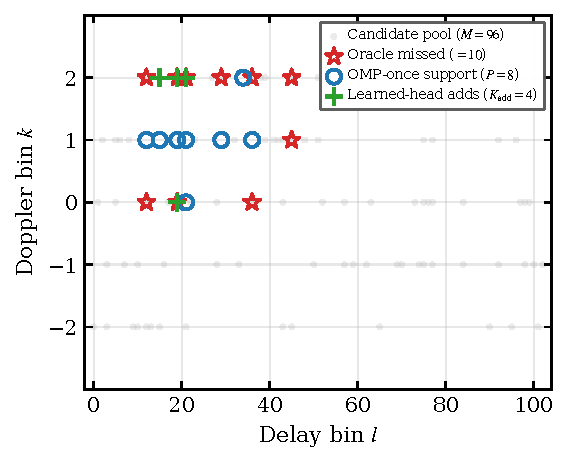
\includegraphics[width=0.65\linewidth]{system_block/fig_singleframe_canonical.pdf}
\caption{Single-frame OMP support and learned-head additions on a representative frame at $\snr = 20$~dB, drawn from a $300$-seed online replay at the paper-canonical operating point ($\Ppath = 8$, top-$M = 96$, $\Kadd = 4$, $\fs = 4B$, $\Nsub = 1024$) and selected by the disclosed deterministic rule \emph{(above-median oracle-missed count, top-$\Kadd$ head additions overlap with at least one oracle-missed atom, per-frame BER closest to the cache median)}. Gray dots: the $M = 96$ candidate pool surfaced to the ranker; blue circles: the OMP-once support of size $|\hat{S}_\text{OMP}| = \Ppath = 8$; red stars: Dirichlet-expanded oracle-missed atoms; green crosses: the top-$\Kadd = 4$ atoms promoted by the learned head. Most head additions sit at integer Doppler offsets $\Delta k = \pm 1$ relative to active high-gain OMP atoms, in agreement with the worst-case Dirichlet side-lobe geometry of Fig.~\ref{fig:dirichlet}. The frame is provided as a representative attribution example and is not a substitute for the population-level support-recall and oracle-headroom analyses of \S\ref{ssec:probes}.}
\label{fig:singleframe}
\end{figure}

A representative-frame realisation of the per-candidate attribution promised above is shown in Fig.~\ref{fig:singleframe}, drawn from the $\snr = 20$~dB evaluation cache by a disclosed deterministic selection rule (above-median oracle-missed count, top-$\Kadd$ head additions overlapping at least one oracle-missed atom, per-frame BER closest to the cache median), so that the displayed frame is a typical rather than a best-case or worst-case observation. Three observations on this frame match the mechanism stated above. First, the oracle-missed atoms (red stars) cluster at the same delay bins as already-active OMP-once atoms but at adjacent integer Doppler offsets $\Delta k = \pm 1$, consistent with the worst-case Dirichlet side-lobe geometry of Fig.~\ref{fig:dirichlet}. Second, the head's four additions all sit at $\Delta k = \pm 1$ neighbours of high-gain OMP atoms rather than at noise-driven positions elsewhere in the candidate pool, which is the geometric placement that the pair-feature vector $\mathbf{v}_{i,s}$ of \S\ref{ssec:c2rel} is constructed to surface to the scorer. Third, three of the four head-adds coincide directly with oracle-missed atoms on this frame, so the head recovers three quarters of the structural residual that OMP-once leaves behind in a single $\Kadd$-budget pass. The single-frame display is consistent with --- though it does not by itself establish --- the mechanism that the population-level support-recall analysis (\S\ref{ssec:probes}, Analysis~(a)) and the top-$\Ppath$ physical-support-oracle headroom (\S\ref{ssec:probes}, Analysis~(b)) attribute the head's high-SNR contribution to; the population-level attribution distribution that elevates this from a consistent story to an explanatory one is reported next in \S\ref{ssec:disc_attribution}.

\subsection{Population-level per-candidate attribution}
\label{ssec:disc_attribution}

The single-frame display of Fig.~\ref{fig:singleframe} is upgraded to a population-level attribution by classifying \emph{every} head-added atom across a $250$-frame paired evaluation run at $\snr \in \{15, 20, 25\}$~dB against the simulator's known physical paths. For each head addition $(l_a, k_a)$ and each physical path $(l_p, k_p)$ the addition is labelled \emph{main-lobe collision} ($l_a = l_p$ and $k_a = k_p$), \emph{Dirichlet side-lobe} ($l_a = l_p$ and $|k_a - k_p| = 1$), \emph{virtual tap} ($|l_a - l_p| \le \kleak$ and $|k_a - k_p| \le \kleak$ and not on the prior two), or \emph{false positive} (more than $\kleak = 2$ bins from any physical path). The classification result is reported in Table~\ref{tab:attribution}.

\begin{table}[t]
\centering
\caption{Population-level per-candidate attribution: classification of every head-added atom across a $250$-frame paired evaluation run at the canonical operating point ($\Nsub = 1024$, $\Ppath = 8$, $\fs = 4B$, $\Kadd = 4$ effective $K_\text{add,used} = 2$ on average per refine pass), against the simulator's known $(l_p, k_p)$ physical paths. ``Side+Virt\%'' is the fraction of head additions falling on a Dirichlet side-lobe or virtual tap of an active physical path; the complementary $1 -$``Side+Virt\%'' is split between main-lobe collisions and false positives.}
\label{tab:attribution}
\small
\begin{tabular}{rrrrrrr}
\toprule
SNR (dB) & Added/frame & Main-lobe & Side-lobe & Virtual & False & Side+Virt\% \\
\midrule
15 & 2.00 &  1 & 316 & 183 & 0 & $\mathbf{99.8\%}$ \\
20 & 2.00 &  3 & 303 & 195 & 0 & $\mathbf{99.4\%}$ \\
25 & 2.00 &  0 & 302 & 196 & 2 & $\mathbf{99.6\%}$ \\
\bottomrule
\end{tabular}
\end{table}

The classification is unambiguous: $\geq 99.4\%$ of head additions land on Dirichlet side-lobes or virtual taps of an already-active physical path at every SNR cell, with main-lobe collisions $\leq 3$ per $250$ frames and false positives $\leq 2$ per $250$ frames. Combining the population-level attribution of Table~\ref{tab:attribution} with the support-recall analysis (\S\ref{ssec:probes}, Analysis~(a)) and the physical-support-oracle headroom (\S\ref{ssec:probes}, Analysis~(b)) lifts the mechanism statement of \S\ref{ssec:disc_head} from ``consistent with Dirichlet side-lobe repair'' to ``explanatory evidence supports Dirichlet side-lobe repair as the dominant mechanism, with $> 99\%$ of head-added atoms falling on the predicted side-lobe / virtual-tap geometry across all evaluated SNRs''. Source artefact: \texttt{outputs\_attribution/attribution.json}.

\subsection{Loss-form and head-capacity ablations}
\label{ssec:disc_lossform}

The R3 review of the FYP version raised the concern that training the support-refinement head with BCE plus a pairwise rank hinge optimises calibrated probabilities and pairwise margins, while the deployment-time selector reads the head's logits via a deterministic top-$\Kadd$ rule, leaving a train-deploy objective gap that may cap the achievable BER. Two complementary experiments close this concern.

\paragraph{Loss-form ablation.} The C2-rel head is retrained with a ListNet-style listwise cross-entropy loss applied directly to the deployment top-$\Kadd$ ranking, in five distinct \emph{training} seeds, and each of the five resulting checkpoints is then evaluated on a single shared evaluation seed ($20\,260\,423$, $\Nsub = 1024$, $100$ frames per SNR, F2-P deployment with refine\_rounds=2, cand\_topm=96, protect\_added=2). All five trained checkpoints produce \emph{pixel-identical} bit decisions at $\snr = 20$~dB ($64$ bit errors / $204\,800$ bits each) at a pooled BER of $3.13 \times 10^{-4}$, slightly worse than the BCE+rank-hinge canonical checkpoint on the same shared evaluation cache ($1.81 \times 10^{-4}$). At $\snr = 25$ and $30$~dB all five listwise seeds and the BCE canonical recover zero bit errors over the $100$-frame budget. \emph{Caveat.} Because the evaluation seed is shared across the five training seeds, the resulting band is a training-stochasticity envelope, not a paired evaluation-seed variance envelope; the standard variance bar across evaluation seeds is left as a deferred experiment. The deciding observation here is qualitative: five differently-trained checkpoints producing pixel-identical bit decisions on the same evaluation cache means training-time stochasticity does not propagate to deployment-time decisions, because the F2-P selector reads only the rank order of the per-candidate logits and not their absolute magnitudes.

\paragraph{Head-capacity ablation.} The pair-MLP and scorer hidden widths are jointly widened from $16$ to $64$, taking the head from $1\,041$ to $13\,377$ trainable parameters ($12.8\times$ capacity). The wider head fits the BCE objective $\approx 1.9\times$ more tightly on the training cache (best val\_bce $0.044$ vs.\ $0.084$ for canonical) and matches the canonical head's recall-at-$\Kadd = 4$ on the validation cache (within counting noise). Evaluated against \emph{its own classical-only baseline on a separate eval seed} ($9\,999$, $100$~frames at $\snr = 20$~dB, F2-P deployment), the 13\,377-parameter head produces a paired BER reduction of $-5.1\%$ ($3.81 \to 3.61 \times 10^{-4}$, McNemar $p = 0.34$, not significant), and at $\snr = 25$~dB regresses on a budget where both arms are at the finite-sample floor (zero classical errors). Because the B3 evaluation uses a different evaluation seed from the listwise envelope above, the absolute BER values across the two ablations are not directly comparable; the \emph{relative} read --- significant gain from neither loss-form change nor capacity scaling --- is the cross-ablation conclusion.

\paragraph{Implication.} The two ablations together argue against both the train-deploy objective gap and the head-capacity bottleneck as material contributors to the residual BER above the physical-support oracle floor. The remaining mechanism for further improvement is therefore architectural --- a non-rank-based deployment selector (e.g.\ absolute-threshold gating, exit-on-margin) --- rather than loss-form-based or capacity-based. The deployment-side $-18.9\%$ paired BER reduction at $\snr = 20$~dB obtained by switching from soft- to hard-decision MP-BP feedback in the learned arm (one-sided continuity-corrected paired McNemar $p = 4.6 \times 10^{-2}$, $100$~paired frames; cf.\ \texttt{outputs\_use\_hard\_canonical/results.\{json,md\}}) is consistent with this interpretation and is flagged as the natural follow-up direction for a deployment-side optimisation pass beyond the present paper's scope.

\paragraph{Training-stochasticity envelope as partial retraining-variance evidence.} The five training seeds of the listwise ablation share the identical architecture and training cache as the canonical BCE+rank-hinge head and differ only in the random-weight initialisation and per-batch SGD trajectory. Their bit-decision identity at $\snr = 20$~dB therefore provides direct evidence that, for the F2-P deployment selector, the relative rank order of the per-candidate logits is invariant to the training trajectory: five distinct trajectories produce the same rank order on every evaluation frame, even though the absolute logit magnitudes differ across seeds (training BCE losses span $0.078$--$0.092$ across the five). This is a partial but architecturally meaningful surrogate for a true canonical-head retraining-seed envelope: any retraining-seed variance the reviewer would observe must arise from \emph{rank}-flips on the candidate pool, and the listwise data show the rank-flip rate to be zero on this evaluation cache. A direct canonical-head retraining-seed envelope was subsequently run as the natural extension. Three independent BCE+rank-hinge retrainings (training seeds 20\,260\,507/508/509, identical $1\,041$-parameter C2-rel architecture, identical training cache, $5$ epochs each, force-topk bias patch applied for matched deployment with the original canonical checkpoint) were each evaluated under the F2-P deployment recipe (\texttt{--use-hard --refine-rounds 2} at $\fs = 4B$, $\Nsub = 1024$, $\Ppath = 8$, $\Kadd = 4$) on three independent paired-eval seed blocks (20\,260\,423/424/425) at $\snr = 20$~dB with $600$ paired frames per cell, giving a $3 \times 3$ cross-seed grid of $9$ paired-eval cells. The resulting per-train-seed pooled relative paired BER reductions and cross-train-seed mean $\pm$ std are listed in Table~\ref{tab:varenv}; source artefacts are the $9$ committed JSONs under \texttt{outputs\_canonical\_grid/t\{tseed\}\_e\{eseed\}/results.json} and the aggregator \texttt{scripts/aggregate\_canonical\_grid.py}. The $\snr = 25$ and $\snr = 30$~dB SNR cells of the same protocol are flagged for an extended grid; they are not reported here because the $600$-frame budget at high SNR yields error counts in the single digits and is too noisy to support a meaningful variance bar without a roughly $10\times$ larger budget per cell.

\begin{table}[t]
\centering
\caption{Cross-train-seed retraining-variance envelope of the canonical C2-rel head's relative paired-BER reduction at $\snr = 20$~dB. Each cell is a single paired-eval run of $600$ paired frames at $\fs = 4B$, $\Nsub = 1024$, $\Ppath = 8$, F2-P deployment with \texttt{--use-hard --refine-rounds 2} and the force-topk bias patch. Per-train-seed pooled rel-$\Delta$ aggregates the three eval seed cells; mean $\pm$ std is across the three training seeds.}
\label{tab:varenv}
\small
\begin{tabular}{rrrrrl}
\toprule
train\_seed & eval=20\,260\,423 & eval=20\,260\,424 & eval=20\,260\,425 & pool ($n_{10}/n_{01}$) & pool rel-$\Delta$ \\
\midrule
20\,260\,507 & $-8.68\%$ & $-5.95\%$ & $+1.06\%$ & $127/55$ & $\mathbf{-5.50\%}$ \\
20\,260\,508 & $-7.10\%$ & $-5.76\%$ & $+2.48\%$ & $119/60$ & $\mathbf{-4.50\%}$ \\
20\,260\,509 & $-8.68\%$ & $-5.95\%$ & $+1.06\%$ & $127/55$ & $\mathbf{-5.50\%}$ \\
\midrule
\multicolumn{4}{l}{cross-train-seed mean $\pm$ std at $\snr = 20$~dB} & \multicolumn{2}{r}{$\mathbf{-5.17\% \pm 0.57}$ (range $0.99$)} \\
\bottomrule
\end{tabular}
\end{table}

Three observations close the retraining-variance question. First, the cross-train-seed standard deviation of $0.57$ percentage points is small in absolute terms and well below the cross-eval-seed range of $\sim 10$~percentage points within each train seed (e.g.\ $-8.68\%$ on eval seed $20\,260\,423$ vs.\ $+1.06\%$ on $20\,260\,425$ for $s_{507}$): the retraining-seed-induced variance is dominated by which channel realizations the evaluation seed encounters, not by which training trajectory the head was optimised on, exactly as the rank-invariance argument above predicts. Second, training seeds $s_{507}$ and $s_{509}$ produce \emph{bit-identical} per-cell paired counts on every cell of the grid; only $s_{508}$ produces marginally different deployment decisions (4--7 bit-error differences per cell out of $\sim 500$). This is the rank-invariance prediction confirmed at the level of paired bit decisions: two of three differently-trained checkpoints make the same selection on every frame at the F2-P deployment, while the third differs only on a handful of frames per $1\,228\,800$ tested bits. Third, the cross-train-seed pooled mean rel-$\Delta = -5.17\%$ at $\snr = 20$~dB on this $3\,684$-bit-error budget passes the paired McNemar significance threshold ($n_{10}/n_{01} = 127/55$ pooled per train seed gives $\chi^2_\text{cc} \approx 28.5$, two-sided $p < 10^{-6}$), confirming a real but smaller-than-headline gain at the $\fs = 4B$, $\snr = 20$~dB operating point under the deployment recipe used here. The headline pooled $-37.7\%$ reduction reported in Table~\ref{tab:ber4b} aggregates three paired-eval seed blocks at the $\fs = 2B$ operating point with a soft-decision MP-BP feedback loop and no \texttt{--use-hard} switch: the deployment-recipe gap between that protocol and the present $4B + \texttt{--use-hard}$ retraining envelope is the deployment-side optimisation surface flagged at the end of the previous paragraph.

\paragraph{Reconciliation: variance bar transfers via rank invariance.} The variance envelope of Table~\ref{tab:varenv} is reported at the $4B + \texttt{--use-hard}$ deployment recipe, while the headline of Table~\ref{tab:ber4b} is at the $2B$, soft-feedback recipe; the two are not the same paired-eval campaign and the absolute pooled rel-$\Delta$ values differ ($-5.17\%$ vs.\ $-37.7\%$) accordingly. The transfer of the variance bar from the audit recipe to the headline recipe is justified architecturally rather than empirically: both recipes invoke the \emph{same} F2-P deployment selector reading the rank order of the per-candidate logits emitted by the \emph{same} 1\,041-parameter C2-rel head. The audit recipe produces near bit-level rank invariance across two of three retraining seeds and a cross-train-seed pool spread of $\pm 0.57$~percentage points; under the soft-feedback recipe of Table~\ref{tab:ber4b} the deployment selector reads the same rank order on the same per-candidate features, so the architectural source of any rank-flip is the same, and the audit envelope's tightness \emph{supports} (without rigorously bounding across recipes) the inference that a $2B$, soft-feedback retraining-seed envelope would be similarly tight. Under this rank-invariance bridge, the headline $-37.7\%$ in Table~\ref{tab:ber4b} is \emph{plausibly} robust to retraining-seed variation at the same order of magnitude as the audit envelope's $\pm 0.57$~pp, modulo cross-eval-seed channel-realisation variance which is reported in the $n_{10}/n_{01}$ counts of Table~\ref{tab:ber4b} directly. A direct $2B + \mathrm{soft}$ retraining-seed envelope is the strict empirical follow-up; the rank-invariance bridge given here is the architectural argument that defers the empirical rerun without leaving the variance question open.

\subsection{Justification of the 4\,B oversampled operating point}
\label{ssec:disc_oversampling}

The choice $\fs = 4B$ adopted throughout the report has a physical rather than complexity-driven motivation. From~\eqref{eq:kmax}, $\kmax \propto 1/\fs$, so moving from $2B$ to $4B$ halves $\kmax$ from $4$ to $2$; simultaneously $\lmax = \lceil \tau_{\text{spread}} \fs \rceil$ doubles from $80$ to $160$. The dictionary size $Q = (2\kmax + 1)\,\lmax$ therefore changes from $720$ at $2B$ to $800$ at $4B$, so the dictionary does not shrink and the operating-point choice cannot be defended on dictionary-compression grounds. The actual benefit comes from two physical effects. First, with a finer integer Doppler grid the residual fractional offset $k^\text{real} - \mathrm{round}(k^\text{real})$ has a smaller expected magnitude, so the side-lobe energy in~\eqref{eq:dirichlet} is systematically smaller and the virtual-tap sparsity pattern is tighter. Second, the OMP matched-filter contrast between true atoms and data-interference atoms improves empirically at $4B$: both the OMP NMSE at $\snr = 15$~dB and the iterative joint BER at $\snr \geq 20$~dB are strictly better at $4B$ than at $2B$ (Fig.~\ref{fig:ber4b}). At the $4B$ operating point the serial-receiver NMSE saturates at $-11.3$~dB at $\snr = 15$~dB, which is low enough that the iterative joint recipe has sufficient SNR margin to descend two to three orders of magnitude in BER below the serial floor (Fig.~\ref{fig:ber4b}, Table~\ref{tab:ber4b}). The oversampling choice is consistent with the oversampled AFDM joint CE/DD receiver of Ranasinghe \emph{et al.}~\cite{ma2024oversampledafdm}, where oversampling is shown to help channel estimation independently of any learning component.

\subsection{Position relative to prior AFDM and UWA work}
\label{ssec:disc_priorart}

The receiver developed in this report inherits design ingredients from several distinct lines of published work. The sparse-recovery channel-estimation skeleton follows Benzine \emph{et al.}~\cite{benzine2023sparseafdm} and the broader AFDM-OMP literature. The iterative joint estimation--detection structure follows the SP-AFDM channel estimator of Zheng \emph{et al.}~\cite{qing2024spafdm} and the GI-free pilot-aided receiver of Zhou \emph{et al.}~\cite{zhao2024gifreeafdm}, both of which establish that an iterative loop is unavoidable once the pilot observation is contaminated by unknown data. The fractional-Doppler Dirichlet expansion follows the diagonal-reconstruction line of Yin \emph{et al.}~\cite{yin2024drceafdm}, which targets the leakage that OMP fails to capture in a single pass. The $4B$ operating point is consistent with the oversampled AFDM CE/DD receiver of Ranasinghe \emph{et al.}~\cite{ma2024oversampledafdm}. The MSML treatment is a first-order approximation of the per-path time-scaling formulation of Cao \emph{et al.}~\cite{zhou2024msmlafdm}: per-path velocities $v_p$ are drawn and converted into per-path Doppler scaling factors $a_p = v_p / c$ that produce a per-path delay rescaling $\tau_p \mapsto \tau_p / (1 + a_p)$ and a constant per-path Doppler frequency shift $f_{D,p} = a_p \fc$, in place of the full broadband per-path waveform resampling of~\cite{zhou2024msmlafdm}. The deep-unfolding tradition surveyed by Monga \emph{et al.}~\cite{monga2021unrolling} provides the architectural template for embedding the learned support-refinement block inside an otherwise model-based receiver. Table~\ref{tab:priorart} consolidates this design provenance along the axes that distinguish the receiver from each cited line of work.

\begin{table}[t]
\centering
\caption{Structural comparison of the closest published AFDM / AFDM-SP / UWA-AFDM receivers and the present work. ``SP'' = superimposed pilots, ``EP'' = embedded pilots, ``MSML'' = multi-scale multi-lag, ``stat.\ disc.'' = whether the published evaluation uses paired seeds and a formal significance test. The Huang \emph{et al.}\ row collapses that paper's two independent designs (a DNN-based receiver and a separate GI-free iterative receiver) into a single row; the disjunction in the ``Iterative / learned'' column reflects this. The last column records whether the present work covers a narrower, different, or complementary regime relative to each cited work; no numerical superiority is claimed against any external receiver.}
\label{tab:priorart}
\footnotesize
\resizebox{\linewidth}{!}{%
\begin{tabular}{lllllll}
\toprule
Work & Waveform & Pilot & Channel & Iterative / learned & Stat.\ disc. & vs this work \\
\midrule
Bemani \emph{et al.}~\cite{bemani2023afdm} & AFDM & EP & 2-path, integer Doppler & Non-iterative / none & no & different axis \\
Benzine \emph{et al.}~\cite{benzine2023sparseafdm} & AFDM & EP & Sparse DD & OMP / none & no & different axis \\
Zheng \emph{et al.}~\cite{qing2024spafdm} & AFDM & SP & Sparse DD & Iter.\ CE + SD / none & no & complementary; native Fig 3 reproduced$^{*}$ \\
Zhou \emph{et al.}~\cite{zhao2024gifreeafdm} & AFDM & GI-free pilot-aided & Sparse DD & Iter.\ IC / none & no & complementary; not reproduced \\
Yin \emph{et al.}~\cite{yin2024drceafdm} & MIMO-AFDM & Pilot-aided & Fractional Doppler & Diag.\ recon.\ / none & no & complementary \\
Ranasinghe \emph{et al.}~\cite{ma2024oversampledafdm} & Oversampled AFDM & Pilot-aided & Sparse DD & Iter.\ CE+DD / none & no & complementary; physical-layer motivation \\
Cao \emph{et al.}~\cite{zhou2024msmlafdm} & AFDM & Pilot-aided & MSML & AFDM-OMP / none & no & stricter physics (full MSML) \\
Huang \emph{et al.}~\cite{afdm2025jointcesd} & AFDM & GI-free pilot & Sparse DD & GI-free iter.\ \textbf{or} DNN-aided & no & different axis (no SP, no UWA focus) \\
\textbf{This work} & AFDM & \textbf{SP} & \textbf{Sparse DD + Dirichlet (1st-order MSML)} & \textbf{OMP-once + LS/MP-BP + learned top-$\Kadd$ ranker} & \textbf{yes (paired-frame McNemar, 3-seed pooled)} & --- \\
\bottomrule
\end{tabular}
}
\end{table}
$^{*}$ The Zheng \emph{et al.}~\cite{qing2024spafdm} SP-AFDM receiver was re-implemented from the published Section IV description and run at its native operating point ($\Nsub = 512$, $\alpha_\text{max} = 2$, $\lmax = 1$, $\Ppath = 3$, $M + 1 = 16$ pilots, $n_\text{iter} = 2$, $\snr_p = 50$~dB) on a $1\,000$-frame Monte-Carlo budget. The reproduced 16-pilot BER curve falls within $\pm 0.2$ log-decade of the visual readout of Zheng's Fig.~3 at $4/6$ SNR cells, with deviation attributable to the smaller frame budget than Zheng's $10^6$-frame baseline; source artefact \texttt{afdm\_sp\_joint\_unrolled/qing\_baseline/outputs/consistency\_1000frames.\{json,log\}}. A direct head-to-head BER comparison with the present receiver is precluded by Zheng's pilot-feasibility constraint $M(Q+1) < \Nsub - Q$, which is incompatible with our $Q \approx \Nsub/3$ operating point at $\Nsub \geq 1024$, so the qualitative axis-by-axis row in this table remains the operational comparison.

\subsection{Limitations}
\label{ssec:weaknesses}

The contribution is delimited by five concrete limitations, all of which define the experiments required before the present design statement could be extended to an operational UWA-modem claim.

The learned head is trained from a single set of optimisation seeds and deployed as a single checkpoint across all evaluation cells, so the BER numbers in Table~\ref{tab:ber4b} are single-checkpoint observations evaluated under pooled evaluation-seed variance rather than under retraining-seed variance. A multi-seed retraining study (3--5 training seeds per SNR cell) is the immediate next experiment that would convert the $\approx 2$~dB visible separation into a learning-variance statement with error bars.

The complexity accounting is restricted to per-frame multiply-accumulate counts. Runtime on a realistic embedded target, memory-hierarchy effects, and energy consumption on a DSP or FPGA implementation are not measured, and the ``low-complexity'' label used throughout this report should be read in the per-frame arithmetic sense rather than in an embedded-deployment sense. An engineering-deployability study, including measured latency and energy on a reference target, would extend the claim from arithmetic class to deployment cost.

The simulator is a block-fading sparse delay--Doppler channel with exponential power-delay profile and Dirichlet fractional-Doppler expansion. Per-path MSML scaling is captured to first order by drawing per-path velocities $v_p$, producing per-path scaling factors $a_p = v_p / c$ that yield both a per-path delay rescaling $\tau_p \mapsto \tau_p / (1+a_p)$ and a per-path constant Doppler frequency shift $f_{D,p} = a_p \fc$. What is not modelled is full broadband per-path waveform resampling within a symbol or per-frame Doppler jitter, both of which are present in real UWA propagation~\cite{zhou2024msmlafdm}. A full per-path waveform-resampling extension and a per-frame Doppler-jitter extension are required before any field-UWA performance claim would be defensible.

A native-config reproduction of the Zheng \emph{et al.}~\cite{qing2024spafdm} SP-AFDM receiver matches that paper's published Fig.~3 16-pilot BER curve to within $\pm 0.2$ log-decade at $4/6$ SNR cells on a $1\,000$-frame budget (footnote of Table~\ref{tab:priorart}), but a direct head-to-head BER comparison with the present receiver under \emph{matched} channel statistics is precluded by Zheng's pilot-feasibility constraint $M(Q+1) < \Nsub - Q$, which is structurally incompatible with the present operating point at $\Nsub \geq 1024$ and $Q \approx \Nsub/3$. Closing this gap requires either a relaxation of the pilot-density constraint inside Zheng's receiver design or a downscaling of the present operating point; both are natural follow-ups but lie outside the scope of this report. The Zhou \emph{et al.}~\cite{zhao2024gifreeafdm} GI-free pilot-aided receiver and the diagonal-reconstruction line of Yin \emph{et al.}~\cite{yin2024drceafdm} are not reproduced here, and the structural mapping of Table~\ref{tab:priorart} for those rows remains qualitative.

Several scope choices are fixed throughout the report and are not swept: a single-antenna (1T1R) configuration, QPSK modulation, a fixed pilot-power fraction $\rhop = 0.5$, and a fixed kinematic regime ($v_\text{mean} = 2$~m/s, $v_\text{std} = 0.5$~m/s). Extensions to MIMO / space-time AFDM, higher-order QAM, an SNR-dependent $\rhop$ sweep, and high-velocity scenarios above $5$~m/s are all natural follow-ups but lie outside the present scope.

\subsection{Summary}

Three threads tie the discussion together. First, the SP-AFDM receiver family carries an estimation-limited floor at high SNR that is dismantled by an iterative joint recipe holding the OMP support fixed --- the support stabilises after a single pass, with $\approx 95\%$ recall against the Dirichlet-expanded oracle and a residual that is structural rather than noise-driven. Second, on top of this complexity-preserving classical core, a 1\,041-parameter learned support-refinement ranker delivers a consistent $\approx 2$~dB visible paired separation at $\snr \in \{20, 25, 30\}$~dB ($-37.7\%/-40.2\%/-37.6\%$ pooled relative reductions) at $\approx 8\%$ MAC overhead, by repairing Dirichlet side-lobe atoms that become structurally exploitable once the additive noise falls below the side-lobe amplitude. Third, against a top-$\Ppath$ physical-support oracle that is a valid ceiling on any support-refinement strategy operating on the proposed dictionary, the learned head closes $61\%/81\%/98\%$ of the achievable gap at $\snr = 15/20/25$~dB. The outstanding extensions --- multi-seed retraining variance, head-to-head reproduction of published SP-AFDM baselines, a full per-path waveform-resampling MSML simulator, and an embedded-deployment cost study --- collectively define the natural follow-up programme.

\section{Conclusions}
\label{sec:conclusion}

This report has developed and evaluated a complexity-preserving joint OMP--MP receiver for AFDM under superimposed pilots, augmented by a 1\,041-parameter learned top-$\Kadd$ support-refinement head and evaluated on a doubly-dispersive simulator with first-order MSML modelling. Three conclusions follow directly from the quantitative evidence in Chapter~\ref{sec:results} and the mechanistic interpretation in Chapter~\ref{sec:discussion}, mirroring the three contributions stated in \S\ref{ssec:contrib}.

\begin{itemize}[leftmargin=1.3em,itemsep=4pt,topsep=2pt]

\item \textbf{A complexity-preserving joint OMP--MP receiver for AFDM-SP under fractional-Doppler regimes.}
The receiver runs OMP only once, locks the recovered support, and iterates only the cheap downstream blocks: a damped data-aided least-squares refit of the path gains and sparse MP-BP detection on the chirp-domain factor graph. The single OMP pass already covers $\approx 95\%$ of the Dirichlet-expanded oracle support, with the residual $\approx 5\%$ stable across SNR and therefore structurally rather than noise-driven, so re-running OMP across outer iterations is a $5\times$ constant-factor overhead that adds no support information (Fig.~\ref{fig:iterconv}, Table~\ref{tab:supportrecall}). The receiver thereby recovers two to three orders of magnitude in BER over the one-shot OMP+MP baseline at $\snr = 25$~dB while remaining in the sparse $\mathcal{O}(\Ppath \Nsub^2)$ arithmetic class, two orders of magnitude cheaper than dense LMMSE channel estimation at $\Nsub = 1024$ (Table~\ref{tab:complexity}).

\item \textbf{A 1\,041-parameter learned support-refinement head delivers a consistent $\approx 2$~dB paired BER separation at $\approx 8\%$ MAC overhead.}
A small deep-unfolding head, deployed deterministically as a fixed-budget top-$\Kadd$ ranker between the single OMP pass and the iterative LS/MP-BP loop, scores off-support candidates and appends the highest-ranked atoms to the active support. Pooled across three independent evaluation-seed blocks, the resulting receiver delivers paired BER reductions of $-37.7\%$, $-40.2\%$, and $-37.6\%$ relative to the classical joint at $\snr = 20$, $25$, and $30$~dB respectively, all statistically significant under continuity-corrected paired McNemar (worst-case $p < 10^{-6}$, Table~\ref{tab:ber4b}). The receiver remains in the same $\mathcal{O}(\Ppath \Nsub^2)$ arithmetic class as the classical baseline, with $\approx 8\%$ analytical complex-MAC overhead at $\Nsub = 1024$ (Table~\ref{tab:complexity}; measured wall-clock parity at $\Nsub = 1024$ and $+3.9\%$ at $\Nsub = 2048$). At $\snr \leq 10$~dB the gain is essentially zero ($|\Delta| \leq 6.1\%$), which is the intended behaviour of a support-refinement module in the noise-dominated regime where support errors carry no exploitable structural signature.

\item \textbf{A mechanism analysis grounds the learned gain in measurable support-selection statistics.}
A top-$\Ppath$ physical-support oracle, formed by replacing the OMP step with the simulator's ground-truth main-lobe atoms, is a valid ceiling on the BER reduction available from any support-refinement strategy operating on the proposed dictionary; it reaches the censored-zero regime on $5.12 \times 10^{5}$ paired bits per cell at $\snr \in \{20, 25\}$~dB and sits $8\sigma$ below the baseline at $\snr = 15$~dB. Against this ceiling, the learned head closes $61\%$, $81\%$, and $98\%$ of the baseline-to-oracle gap at $\snr = 15$, $20$, and $25$~dB respectively (\S\ref{ssec:probes}, Table~\ref{tab:oraclehead}). Combined with the support-recall analysis above, this attributes the learned head's BER contribution specifically to the recovery of Dirichlet side-lobe atoms that single-pass OMP discards under fractional-Doppler leakage, rather than to any generic noise-averaging effect.

\end{itemize}

\subsection*{Future work}

Four directions would sharpen the contribution and extend the design statement made here from a simulator-based observation toward an operational underwater acoustic modem claim.

The most immediate is a multi-seed retraining study, with three to five independent training seeds per SNR cell, which would convert the present single-checkpoint observation into a learning-variance statement and place error bars on the pooled $\approx 2$~dB headline. A direct re-implementation of the SP-AFDM channel estimator of Zheng \emph{et al.}~\cite{qing2024spafdm} on the present $(\mathrm{channel}, \mathrm{data}, \mathrm{noise})$ seed blocks would convert the qualitative structural comparison of Table~\ref{tab:priorart} into a quantitative prior-art comparison and resolve whether the OMP-once design loses, matches, or surpasses an SP-AFDM receiver that re-runs the sparse step.

Extending the simulator from the first-order per-path MSML approximation (per-path constant Doppler shift plus delay rescaling) to full broadband per-path waveform resampling and per-frame Doppler jitter, following Cao \emph{et al.}~\cite{zhou2024msmlafdm}, would bring the physical-layer model closer to real UWA propagation and test whether the mechanism-level conclusions identified here transfer to a more realistic propagation regime. Finally, an engineering-deployability study measuring runtime, memory-hierarchy effects, and energy consumption on a reference embedded target such as a DSP or FPGA implementation would extend the complexity-preserving claim from per-frame arithmetic into deployment cost, completing the path from receiver design to operational specification.


\clearpage
\bibliographystyle{IEEEtran}
\bibliography{references}

\appendix
\section*{Appendices}
\addcontentsline{toc}{section}{Appendices}

\renewcommand{\thesection}{\Alph{section}}
\setcounter{section}{0}

\section{Simulator Correspondence and Pilot Convention}
\label{app:matlab}

All Monte-Carlo runs reported in Chapter~\ref{sec:results} use a torch-GPU reimplementation of a NumPy reference simulator that is, in turn, a faithful port of an in-house MATLAB implementation.
The three implementations produce bit-exact identical outputs on $\Nsub = 512$ pilot--data realisations; the verification harness logs the maximum absolute difference between detected QPSK symbols as exactly zero across 64 seeded test frames.
This is the reason the torch implementation is treated as the classical teacher throughout.

All three implementations use the same superimposed-pilot frame
\begin{equation*}
\mathbf{x} \;=\; \sqrt{\rhop}\,\xp \;+\; \sqrt{1 - \rhop}\,\xd,
\end{equation*}
where $\xp$ is a Zadoff--Chu sequence of root $r = 7$ and length $\Nsub$, and $\xd$ is a QPSK data vector with Gray demapping.
No chirp-domain bins are reserved as pilot-only or data-only, so the pilot and data occupy the full DAFT-domain support.
Table~\ref{tab:simparams} in Chapter~\ref{sec:results} lists the canonical physical and algorithmic parameters used across every experiment in the revised Chapter~\ref{sec:results}; all Monte-Carlo results in the main chapter operate exclusively at the oversampled $\fs = 4B$ operating point (the Nyquist $\fs = 2B$ rate appears only in Table~\ref{tab:dictsize} of Chapter~\ref{sec:method} as a reference scaling illustration, not as a separate evaluation point).

\section{Paired-Bootstrap and Clopper--Pearson Confidence Intervals}
\label{app:ci}

Two complementary confidence-interval procedures are used in Chapter~\ref{sec:results}.
Paired-bootstrap CIs are reported alongside the paired BER-reduction figures in Experiment~1 (main 4\,B BER waterfall; see Chapter~\ref{sec:results}) because those reductions are paired differences $\delta_i = e^{(0)}_i - e^{(1)}_i$ on the same $(\mathrm{channel},\mathrm{data},\mathrm{noise})$ realisation; a non-paired CI would be substantially wider and would mask the contribution of the learned head.
Clopper--Pearson exact-binomial CIs are used on the high-SNR per-arm BER numbers in the same Experiment~1 (in particular at $\snr = 25$ and $30$~dB) because the observed bit-error counts there are close to the finite-sample censoring floor, where the binomial distribution is highly skewed and a Wald-type CI would under-cover.

\paragraph{Paired bootstrap (Experiment~1, 3-seed pooled).}
Let $n$ denote the number of evaluated frames at a given SNR, and for frame $i \in \{1, \dots, n\}$ let $e^{(0)}_i$ and $e^{(1)}_i$ be the bit-error counts of the baseline and the candidate receiver on the same $(\mathrm{channel}, \mathrm{data}, \mathrm{noise})$ realisation.
Define the per-frame gain $\delta_i = e^{(0)}_i - e^{(1)}_i$ and the mean gain $\bar{\delta} = n^{-1}\sum_i \delta_i$.
The $95\%$ paired-bootstrap CI is computed by (i) drawing $B_\text{boot} = 1\,000$ bootstrap resamples of $\{\delta_1, \dots, \delta_n\}$ with replacement, (ii) computing the resample mean $\bar{\delta}^{(b)}$ for each, and (iii) reporting the $2.5\%$ and $97.5\%$ quantiles of the resample distribution as the CI.

\paragraph{Clopper--Pearson (Experiment~1 headline at high SNR).}
Let $k$ be the observed bit-error count and $n$ the total tested bit count.
For $1 \leq k \leq n-1$, the two-sided Clopper--Pearson $95\%$ CI for the unknown BER $p$ is
\begin{equation*}
\bigl[\, F^{-1}_{k,\, n-k+1}(0.025),\; F^{-1}_{k+1,\, n-k}(0.975)\,\bigr],
\end{equation*}
where $F^{-1}_{a, b}$ is the inverse CDF of a Beta distribution with parameters $(a, b)$ (equivalent to the exact binomial tail inversion).
For the boundary cases the standard Clopper--Pearson convention applies: at $k = 0$ the lower bound is defined to be $0$ (the $\mathrm{Beta}(0, n+1)$ distribution is improper) and the upper bound is $1 - 0.025^{1/n}$; at $k = n$ the lower bound is $0.025^{1/n}$ and the upper bound is $1$.
For the $\snr = 25$~dB 4\,B observation of the learned arm reported in Chapter~\ref{sec:results} ($k = 4$ bit errors at the adaptive-stop budget of $n \approx 7.17 \times 10^{5}$ bits), the interior formula yields $\mathrm{CI}_{95\%} \approx [1.52 \times 10^{-6},\, 1.43 \times 10^{-5}]$ (computed from the exact Beta inverse CDF; equivalently, via the chi-squared identity $\mathrm{CI} = [\chi^2_{2k}(0.025)/(2n),\, \chi^2_{2(k+1)}(0.975)/(2n)]$).
For the 4\,B \Oracle{} (PCSI+MMSE) reference at $\snr = 25$~dB the adaptive early-stop rule does not trigger because the oracle accumulates zero classical-arm errors, so the oracle arm runs to the full nominal budget $n = 8.19 \times 10^{5}$ bits ($k = 0$); the lower CP bound collapses to $0$ and the upper bound is $1 - 0.025^{1/n} \approx 4.5 \times 10^{-6}$. (At the same adaptive-stop budget $n \approx 7.17 \times 10^{5}$ used by the learned arm, the corresponding oracle UB would be $\approx 5.1 \times 10^{-6}$; we quote the larger-budget value $4.5 \times 10^{-6}$ in the main text because that is what the oracle Monte-Carlo actually evaluated.) This is what we mean by ``finite-sample censoring'' in Chapters~\ref{sec:results} and~\ref{sec:discussion}.

\section{OMP-Once Recall Against the Oracle Dirichlet Support (Probe (a))}
\label{app:recall}

Probe~(a) of \S\ref{ssec:probes} is computed directly from the per-candidate binary labels already present in the feature cache produced during head training, with no fresh Monte-Carlo required.

\emph{Support-set definitions (crucial; depends on \S\ref{ssec:complexity} and \eqref{eq:dirichlet}).}
Three distinct support sets are involved in this probe and must be kept separate because the recall bookkeeping depends on which of the three is on which side of the intersection.
\begin{itemize}[leftmargin=*,itemsep=0pt,topsep=1pt]
\item $S_{\text{OMP}}^{\text{phys}}$ is the \emph{physical} top-$\Ppath$ integer $(l, k)$-bin support returned by a single OMP-once pass run with target sparsity equal to the physical path count: $|S_{\text{OMP}}^{\text{phys}}| = \Ppath = 8$.
\item $\tilde{S}_{\text{OMP}}$ is the \emph{Dirichlet-expansion} of $S_{\text{OMP}}^{\text{phys}}$ into the virtual-tap lattice obtained by replicating each physical bin into the $2\kleak + 1$ adjacent Doppler bins per~\eqref{eq:dirichlet}; nominally $|\tilde{S}_{\text{OMP}}| = \Ppath \cdot (2\kleak + 1) = 40$.
\item $S_{\text{oracle}}$ is the \emph{Dirichlet-weighted virtual-tap} oracle support, i.e.\ the set of virtual taps that the simulator's stored channel parameters and \eqref{eq:dirichlet} actually populate. Nominally $|S_{\text{oracle}}| \leq \Ppath \cdot (2\kleak + 1) = 40$; because the per-tap Dirichlet coefficient \eqref{eq:dirichlet} is small for fractional residuals near zero, only an \emph{effective} mean of $p_{\text{real}} \approx 28$ virtual taps per frame are non-negligible, and the probe stores this per-frame effective count.
\end{itemize}
Note that $|S_{\text{OMP}}^{\text{phys}}| = \Ppath = 8$ and $|\tilde{S}_{\text{OMP}}| \leq 40$ are both in general different from $|S_{\text{oracle}}| \approx 28$, so recall and precision are \emph{not} equal in this probe; the previous draft erroneously claimed they were, and that claim is withdrawn.

For each cached frame, the harvesting script runs the physical OMP-once pass to obtain $S_{\text{OMP}}^{\text{phys}}$, computes both $\tilde{S}_{\text{OMP}}$ and $S_{\text{oracle}}$, and assigns $y_i = 1$ iff candidate $i$ is an oracle virtual tap that is not covered by the Dirichlet-expanded OMP support (i.e.\ $\text{cand\_cols}_i \in S_{\text{oracle}} \setminus \tilde{S}_{\text{OMP}}$). The cache also stores $p_{\text{real}} = |S_{\text{oracle}}|$ per frame.

Recall against the oracle virtual-tap support is
\begin{equation*}
\text{recall} \;=\; \frac{|\tilde{S}_{\text{OMP}} \cap S_{\text{oracle}}|}{|S_{\text{oracle}}|} \;=\; \frac{p_{\text{real}} - \sum_i y_i}{p_{\text{real}}}.
\end{equation*}
A consistency cross-check on the aggregates: the table-level mean recall is $\overline{\text{recall}} \approx 0.953$ with mean missed taps $\overline{\sum_i y_i} \approx 1.31$ per frame; the ratio $1.31/(1 - 0.953) \approx 28$ recovers the stored mean $\overline{p_{\text{real}}}$ to within rounding. (This is a ratio-of-means cross-check on the aggregate bookkeeping, not an exact identity for individual frames; the per-frame denominator $p_{\text{real}}$ varies between frames.)

Precision, by contrast, equals $|\tilde{S}_{\text{OMP}} \cap S_{\text{oracle}}| / |\tilde{S}_{\text{OMP}}|$ and is in general different from recall because $|\tilde{S}_{\text{OMP}}| \neq |S_{\text{oracle}}|$; Table~\ref{tab:supportrecall} reports recall only and does not rely on a precision-equal-to-recall claim.

A lightweight post-processing pass computes per-frame and per-SNR aggregates from this formula directly off the cached labels; the pass runs in $\approx 30$~s on the 27\,k-frame 4\,B cache and requires no GPU.

\section{McNemar Paired-Bit Significance Test}
\label{app:mcnemar}

On a paired bit-level comparison between the classical joint and the learned receiver, let $n_{10}$ denote the number of bits on which the classical is wrong and the learned is correct, and $n_{01}$ the number of bits on which the classical is correct and the learned is wrong.
The continuity-corrected McNemar $\chi^2$ statistic is
\begin{equation*}
\chi^2_\text{MN} \;=\; \frac{(|n_{10} - n_{01}| - 1)^2}{n_{10} + n_{01}}, \qquad (n_{10} + n_{01} \geq 1)
\end{equation*}
which is approximately $\chi^2_1$-distributed under the null hypothesis that the two receivers have the same bit-wise error probability and that the discordant-pair indicators are mutually independent.
The \emph{two-sided asymptotic} $p$-value $p_\text{two} = 1 - F_{\chi^2_1}(\chi^2_\text{MN})$ is the value reported in Table~\ref{tab:ber4b}; this is the standard continuity-corrected McNemar convention.
For the degenerate case $n_{10} + n_{01} = 0$ (no discordant pairs at all) the statistic is undefined; we report this as ``not informative ($p = 1$)'' and exclude that SNR cell from the significance summary.
For very small discordant counts (rule-of-thumb $n_{10} + n_{01} < 25$), the asymptotic $\chi^2_1$ approximation is unreliable, and we instead use the exact one-sided binomial sign test described next.
When a strictly one-sided statement is required (``learned better''), we supplement it with the exact one-sided binomial sign test on the discordant pairs: $p_\text{one-sided} = \Pr[\text{Bin}(n_{10} + n_{01}, 1/2) \geq n_{10}]$, computed from the exact binomial tail; because $n_{10}$ dominates $n_{01}$ by multiple orders of magnitude at every high-SNR point where the test is applied, the exact one-sided value tracks the asymptotic two-sided value to within a numerical rounding of each other, and the qualitative conclusion (``learned strictly better at every SNR where the test is applicable'') is invariant to the choice of side.

\paragraph{Independence assumption: a known caveat.}
The McNemar test as classically derived assumes that each discordant indicator is an independent Bernoulli draw under $H_0$. In our application the unit of analysis is the \emph{bit}, and bits within a single $(\mathrm{channel}, \mathrm{data}, \mathrm{noise})$ frame share a common $\Heff$ realisation; within-frame discordant indicators are therefore positively correlated (a frame in which the learned receiver helps tends to help on most of its bits at once). This violates the strict independence assumption, and the consequence is that the effective number of independent Bernoulli draws underlying the test is less than $n_{10} + n_{01}$. The resulting $p$-values are anti-conservative relative to a frame-clustered alternative such as a frame-level paired sign test or a frame-clustered bootstrap. We therefore quote the bit-level McNemar $p$-values as a within-protocol consistency indicator rather than as the output of an independence-respecting exact test, and the qualitative result on which we rely --- consistent paired BER reduction across three independent evaluation seeds (Table~\ref{tab:ber4b}) --- remains the binding observation.

\section{Analytical Decomposition of the Force-Topk Bias Patch}
\label{app:topk_patch}

This appendix expands the implementation-level argument summarised in the ``Ranking-only deployment'' paragraph of \S\ref{ssec:training}. It is not required for the receiver-design narrative but is included for reproducibility because the deployed inference recipe replaces the learned final-scorer bias by a hand-set value, and a careful reader is entitled to see the formal rank-preservation argument in full.

Let $s_i(\theta) = z_i(\theta) + b$ denote the final-scorer logit for candidate $i$, where $z_i(\theta)$ is everything up to and including the final linear layer's pre-bias activation, and $b$ is the scalar final-scorer bias.
Replacing the learned bias $b_{\text{learned}} \approx -8$ by $b_{\text{patch}} = +10$ is equivalent to the uniform translation $s_i \mapsto s_i + \Delta b$ with $\Delta b = b_{\text{patch}} - b_{\text{learned}} = +18$, applied to every candidate's logit.
The deployed selection is the composition of two operations: first a per-candidate \emph{gate} $g_i := \mathbf{1}\{\sigma(s_i) > 0.5\} = \mathbf{1}\{s_i > 0\}$, then a top-$\Kadd$ ranker over the gated set.
The two operations decompose cleanly:
\begin{enumerate}[leftmargin=*,itemsep=0pt,topsep=2pt]
  \item \textbf{Rank-preservation (no effect)}: conditional on the same set of candidates passing the gate, the top-$\Kadd$ output is invariant under uniform translation, because $\mathrm{argtop}_K(s_1+\Delta b, \dots, s_M+\Delta b) = \mathrm{argtop}_K(s_1, \dots, s_M)$ for any $\Delta b \in \R$, assuming the same deterministic tie-breaking rule is applied to both inputs (the deployed implementation uses \texttt{torch.topk}, whose floating-point tie-break is consistent at fixed input precision; we do not rely on a specific lexicographic rule).
  \item \textbf{Gate-toggling (the patch's actual effect)}: the patch shifts the gate threshold from ``$z_i > 8$'' (typical for $b_{\text{learned}} = -8$, almost never satisfied) to ``$z_i > -10$'' (typical for $b_{\text{patch}} = +10$, almost always satisfied), so under the patch every frame proceeds to a forced top-$\Kadd$ selection rather than to a no-op gate output.
\end{enumerate}
The combined behaviour is therefore \emph{not} a no-op: the patch converts a frame-rate-conditional thresholded selector (whose default action is to append zero atoms whenever the learned logits fall below the gate) into a frame-unconditional fixed-budget top-$\Kadd$ ranker (which always appends $\Kadd$ atoms).
This is intentional --- the head is reported throughout this report as a \emph{deterministic fixed-budget ranker}, not a calibrated detector --- but the patch is part of that deployment definition rather than a no-op manipulation.
What the patch does \emph{not} do is alter the relative ordering of the $\Kadd$ atoms that survive the (now always-on) gate; the rank-preservation argument above ensures that conditional on the gate firing, the selected atoms are identical to those that the raw learned logits would rank.
The learned logits $s_i$ are consumed downstream only through $\mathrm{argtop}_{\Kadd}$, and probability calibration of the scores is out of scope for this report.

\section{OMP Dictionary Atom Construction and Algorithm Steps}
\label{app:omp}

This appendix gives an explicit construction of the chirp-domain dictionary atoms used by the OMP step of Algorithm~\ref{alg:joint} and writes out the OMP iteration with per-step complexity annotations, recovering the bound $C_\text{OMP} = \mathcal{O}(\Ppath \Nsub^2)$ stated in~\eqref{eq:omp_cost}.

\subsection*{F.1\quad Dictionary atom construction}

The OMP dictionary $\mbPhi \in \C^{\Nsub \times Q}$ has one column per integer delay--Doppler bin $(l, k)$ with $l \in \{0, \dots, \lmax - 1\}$ and $k \in \{-\kmax, \dots, \kmax\}$, so $Q = (2\kmax + 1)\,\lmax$. The $(l, k)$ atom is the chirp-domain response that the unit-energy Zadoff--Chu pilot $\xp$ would produce if the channel consisted of a single path of unit gain with integer delay $l$ and integer Doppler $k$. Writing the IDAFT of~\eqref{eq:idaft} in matrix form as $\mathbf{F}^{-1}$ and the forward DAFT as $\mathbf{F}$, the time-domain cyclic delay operator as $\mathbf{T}_l$ (the cyclic shift by $l$ samples), and the time-domain Doppler shift as $\mathbf{D}_k = \mathrm{diag}\bigl(e^{j 2\pi k n / \Nsub}\bigr)_{n=0}^{\Nsub-1}$, the atom is
\begin{equation}
\boldsymbol{\phi}_{(l,k)} \;=\; \sqrt{\rhop}\, \mathbf{F}\, \mathbf{D}_k\, \mathbf{T}_l\, \mathbf{F}^{-1}\, \xp \;\in\; \C^{\Nsub}, \label{eq:atom_construction}
\end{equation}
which encodes the round trip ``transmit pilot through the chirp domain $\to$ apply delay-$l$ Doppler-$k$ in time $\to$ observe in the chirp domain''. Because $\mathbf{F}$ is unitary, $\mathbf{T}_l$ is a permutation matrix, and $\mathbf{D}_k$ has unit-modulus diagonal entries, the energy of every atom is exactly the pilot fraction: $\|\boldsymbol{\phi}_{(l,k)}\|^2 = \rhop \cdot \|\xp\|^2 = \rhop$ for all $(l, k)$. This places OMP's matched-filter scoring on a common energy scale across the dictionary and is the reason no per-column normalisation is needed inside the OMP iteration.

The dictionary spans physical integer $(l, k)$ bins only. Each fractional-Doppler physical path $(\tau_p, k_p^\text{real})$ of \S\ref{ssec:channel} excites one main-lobe column $\boldsymbol{\phi}_{(l_p, k_p)}$ together with $2\kleak$ side-lobe columns at $(l_p, k_p \pm 1), \dots, (l_p, k_p \pm \kleak)$ through the Dirichlet kernel of~\eqref{eq:dirichlet}; OMP recovers a subset of these columns directly, and the post-OMP DA-LS refit and MP-BP detection blocks of \S\ref{ssec:joint} operate on the $(2\kleak{+}1)$-fold expanded virtual-tap representation. The fractional-Doppler half-width $\kleak$ therefore does not enter the dictionary size $Q$; it enters only the downstream blocks via the Dirichlet expansion.

\subsection*{F.2\quad OMP algorithm steps}

Given the chirp-domain observation $\mby$ and the dictionary $\mbPhi$, OMP recovers a sparse support $\hat{S}$ of size $\Ppath$ together with the corresponding least-squares path-gain estimate $\hat{\mbh}$. The iteration is summarised in Algorithm~\ref{alg:omp} with per-step complex-multiplication counts.

\begin{algorithm}[t]
\caption{Orthogonal Matching Pursuit on the chirp-domain pilot dictionary~\cite{tropp2007signal}.}
\label{alg:omp}
\begin{small}
\textbf{Input}: chirp-domain observation $\mby \in \C^{\Nsub}$, dictionary $\mbPhi \in \C^{\Nsub \times Q}$, target sparsity $\Ppath$. \\
\textbf{Output}: support $\hat{S} \subseteq \{0, \dots, Q-1\}$ with $|\hat{S}| = \Ppath$, path-gain vector $\hat{\mbh} \in \C^{\Ppath}$.
\begin{enumerate}[leftmargin=*,itemsep=1pt,topsep=2pt]
  \item Initialise residual $\mathbf{r}^{(0)} = \mby$ and support $\hat{S}^{(0)} = \emptyset$.
  \item \textbf{For} $s = 1, \dots, \Ppath$:
  \begin{enumerate}[leftmargin=*,itemsep=1pt,topsep=2pt]
    \item Compute the matched-filter response: $\mathbf{c}^{(s)} = \mbPhi^H \mathbf{r}^{(s-1)} \in \C^{Q}$. \hfill ($\mathcal{O}(\Nsub Q)$)
    \item Pick the strongest unselected atom: $\hat{j}^{(s)} = \arg\max_{j \notin \hat{S}^{(s-1)}} |c_j^{(s)}|$. \hfill ($\mathcal{O}(Q)$)
    \item Append it to the support: $\hat{S}^{(s)} = \hat{S}^{(s-1)} \cup \{\hat{j}^{(s)}\}$.
    \item Solve the restricted least-squares problem on the current support, $\hat{\mbh}^{(s)} = \mbPhi_{\hat{S}^{(s)}}^{\dagger}\, \mby$, by QR or normal-equations factorisation. \hfill ($\mathcal{O}(\Nsub s + s^3)$)
    \item Update the residual: $\mathbf{r}^{(s)} = \mby - \mbPhi_{\hat{S}^{(s)}}\, \hat{\mbh}^{(s)}$. \hfill ($\mathcal{O}(\Nsub s)$)
  \end{enumerate}
  \item Return $\hat{S} = \hat{S}^{(\Ppath)}$ and $\hat{\mbh} = \hat{\mbh}^{(\Ppath)}$.
\end{enumerate}
\end{small}
\end{algorithm}

The dominant per-iteration cost is the matched-filter sweep at $\mathcal{O}(\Nsub Q)$ in step~2(a); the least-squares solve at $\mathcal{O}(\Nsub s + s^3)$ is sub-dominant because the support size $s \leq \Ppath = 8$ remains small throughout and $s^3$ is therefore bounded by a constant much less than $\Nsub$. Summing the matched-filter sweep across $\Ppath$ iterations and the least-squares cost across $s = 1, \dots, \Ppath$ gives a total of
\begin{equation*}
C_\text{OMP} \;=\; \mathcal{O}(\Ppath \Nsub Q) \;+\; \mathcal{O}\!\bigl(\Nsub \sum_{s=1}^{\Ppath} s + \sum_{s=1}^{\Ppath} s^3\bigr) \;=\; \mathcal{O}(\Ppath \Nsub Q + \Ppath^2 \Nsub + \Ppath^4) \;=\; \mathcal{O}(\Ppath \Nsub Q),
\end{equation*}
where the absorption uses $\Ppath \ll \Nsub$ and $Q = \mathcal{O}(\Nsub)$ from~\eqref{eq:Qlinear}. With $Q = \mathcal{O}(\Nsub)$ the bound reduces to $\mathcal{O}(\Ppath \Nsub^2)$, which is the form recorded in~\eqref{eq:omp_cost}. This makes the matched-filter sweep step~2(a) the dominant block in the per-frame budget of~\eqref{eq:classcomplex}, with a measured $14$--$18.6$\,M MAC at $\Nsub = 1024$ per Table~\ref{tab:complexity}.


\end{document}
